%\documentclass{scrbook}
% Generated by Sphinx.
\def\sphinxdocclass{report}
\documentclass[a4paper,11pt,english]{sphinxmanual}
\usepackage[utf8]{inputenc}
\DeclareUnicodeCharacter{00A0}{\nobreakspace}
\usepackage{cmap}
\usepackage[T1]{fontenc}
\usepackage{babel}
%\usepackage{times}
\usepackage[Sonny]{fncychap}
\usepackage{longtable}
\usepackage{sphinx}
\usepackage{multirow}
\usepackage{amsmath}
\usepackage{amssymb}

\usepackage{titlesec}
\usepackage{verbatim}
\usepackage{textcomp}

\addto\captionsenglish{\renewcommand{\figurename}{Fig. }}
\addto\captionsenglish{\renewcommand{\tablename}{Table }}
\floatname{literal-block}{Listing }

\titleformat{\part}[display]
  {\normalfont\sffamily\huge\bfseries\color{black}}
  {\partname\ \thepart}{20pt}{\Huge}

\title{DFTB$^{\text{+}}$XT Guide \\ version 1.02}

\release{(Development) \today} 
%\release{January 18, 2018}
\author{}
\newcommand{\sphinxlogo}{}
\renewcommand{\releasename}{Release}

\newcommand{\dftbp}{\textsf{DFTB$^{\text{+}}$\ }} %% noodle (alias dftb+)
\newcommand{\dftbpa}{\textsf{DFTB$^{\text{+}}$}} %% noodle (alias dftb+)
\newcommand{\dftbpxt}{\textsf{DFTB$^{\text{+}}$XT\ }} %% noodle (alias dftb+xt)
\newcommand{\dftbpxta}{\textsf{DFTB$^{\text{+}}$XT}} %% noodle (alias dftb+xt)

\newcommand{\cb}{\{\}}  
\newcommand{\is}[1]{{\sffamily{#1}}}            
\newcommand{\iscb}[1]{\is{#1\cb}}
\makeatletter
\newcommand{\verbatimfont}[1]{\def\verbatim@font{#1}}%
\makeatother
\verbatimfont{\sf}

\date{\normalfont\sffamily {http://quantranspro.org/dftb+xt/}\\[0.2cm]
  detailed description of input and output is given in the \dftbpxt USER MANUAL \\[0.2cm]
  this guide focuses on quantum transport \\
  please go to {http://dftbplus.org/} for additional \dftbp documentation}

\makeindex

\makeatletter
\def\PYG@reset{\let\PYG@it=\relax \let\PYG@bf=\relax%
    \let\PYG@ul=\relax \let\PYG@tc=\relax%
    \let\PYG@bc=\relax \let\PYG@ff=\relax}
\def\PYG@tok#1{\csname PYG@tok@#1\endcsname}
\def\PYG@toks#1+{\ifx\relax#1\empty\else%
    \PYG@tok{#1}\expandafter\PYG@toks\fi}
\def\PYG@do#1{\PYG@bc{\PYG@tc{\PYG@ul{%
    \PYG@it{\PYG@bf{\PYG@ff{#1}}}}}}}
\def\PYG#1#2{\PYG@reset\PYG@toks#1+\relax+\PYG@do{#2}}

\expandafter\def\csname PYG@tok@m\endcsname{\def\PYG@tc##1{\textcolor[rgb]{0.13,0.50,0.31}{##1}}}
\expandafter\def\csname PYG@tok@ss\endcsname{\def\PYG@tc##1{\textcolor[rgb]{0.32,0.47,0.09}{##1}}}
\expandafter\def\csname PYG@tok@mi\endcsname{\def\PYG@tc##1{\textcolor[rgb]{0.13,0.50,0.31}{##1}}}
\expandafter\def\csname PYG@tok@gr\endcsname{\def\PYG@tc##1{\textcolor[rgb]{1.00,0.00,0.00}{##1}}}
\expandafter\def\csname PYG@tok@se\endcsname{\let\PYG@bf=\textbf\def\PYG@tc##1{\textcolor[rgb]{0.25,0.44,0.63}{##1}}}
\expandafter\def\csname PYG@tok@s\endcsname{\def\PYG@tc##1{\textcolor[rgb]{0.25,0.44,0.63}{##1}}}
\expandafter\def\csname PYG@tok@sr\endcsname{\def\PYG@tc##1{\textcolor[rgb]{0.14,0.33,0.53}{##1}}}
\expandafter\def\csname PYG@tok@sh\endcsname{\def\PYG@tc##1{\textcolor[rgb]{0.25,0.44,0.63}{##1}}}
\expandafter\def\csname PYG@tok@vi\endcsname{\def\PYG@tc##1{\textcolor[rgb]{0.73,0.38,0.84}{##1}}}
\expandafter\def\csname PYG@tok@sb\endcsname{\def\PYG@tc##1{\textcolor[rgb]{0.25,0.44,0.63}{##1}}}
\expandafter\def\csname PYG@tok@vc\endcsname{\def\PYG@tc##1{\textcolor[rgb]{0.73,0.38,0.84}{##1}}}
\expandafter\def\csname PYG@tok@kd\endcsname{\let\PYG@bf=\textbf\def\PYG@tc##1{\textcolor[rgb]{0.00,0.44,0.13}{##1}}}
\expandafter\def\csname PYG@tok@cp\endcsname{\def\PYG@tc##1{\textcolor[rgb]{0.00,0.44,0.13}{##1}}}
\expandafter\def\csname PYG@tok@bp\endcsname{\def\PYG@tc##1{\textcolor[rgb]{0.00,0.44,0.13}{##1}}}
\expandafter\def\csname PYG@tok@il\endcsname{\def\PYG@tc##1{\textcolor[rgb]{0.13,0.50,0.31}{##1}}}
\expandafter\def\csname PYG@tok@nn\endcsname{\let\PYG@bf=\textbf\def\PYG@tc##1{\textcolor[rgb]{0.05,0.52,0.71}{##1}}}
\expandafter\def\csname PYG@tok@s1\endcsname{\def\PYG@tc##1{\textcolor[rgb]{0.25,0.44,0.63}{##1}}}
\expandafter\def\csname PYG@tok@mh\endcsname{\def\PYG@tc##1{\textcolor[rgb]{0.13,0.50,0.31}{##1}}}
\expandafter\def\csname PYG@tok@si\endcsname{\let\PYG@it=\textit\def\PYG@tc##1{\textcolor[rgb]{0.44,0.63,0.82}{##1}}}
\expandafter\def\csname PYG@tok@sc\endcsname{\def\PYG@tc##1{\textcolor[rgb]{0.25,0.44,0.63}{##1}}}
\expandafter\def\csname PYG@tok@cpf\endcsname{\let\PYG@it=\textit\def\PYG@tc##1{\textcolor[rgb]{0.25,0.50,0.56}{##1}}}
\expandafter\def\csname PYG@tok@w\endcsname{\def\PYG@tc##1{\textcolor[rgb]{0.73,0.73,0.73}{##1}}}
\expandafter\def\csname PYG@tok@ge\endcsname{\let\PYG@it=\textit}
\expandafter\def\csname PYG@tok@gp\endcsname{\let\PYG@bf=\textbf\def\PYG@tc##1{\textcolor[rgb]{0.78,0.36,0.04}{##1}}}
\expandafter\def\csname PYG@tok@go\endcsname{\def\PYG@tc##1{\textcolor[rgb]{0.20,0.20,0.20}{##1}}}
\expandafter\def\csname PYG@tok@sd\endcsname{\let\PYG@it=\textit\def\PYG@tc##1{\textcolor[rgb]{0.25,0.44,0.63}{##1}}}
\expandafter\def\csname PYG@tok@nt\endcsname{\let\PYG@bf=\textbf\def\PYG@tc##1{\textcolor[rgb]{0.02,0.16,0.45}{##1}}}
\expandafter\def\csname PYG@tok@mf\endcsname{\def\PYG@tc##1{\textcolor[rgb]{0.13,0.50,0.31}{##1}}}
\expandafter\def\csname PYG@tok@kc\endcsname{\let\PYG@bf=\textbf\def\PYG@tc##1{\textcolor[rgb]{0.00,0.44,0.13}{##1}}}
\expandafter\def\csname PYG@tok@kn\endcsname{\let\PYG@bf=\textbf\def\PYG@tc##1{\textcolor[rgb]{0.00,0.44,0.13}{##1}}}
\expandafter\def\csname PYG@tok@vg\endcsname{\def\PYG@tc##1{\textcolor[rgb]{0.73,0.38,0.84}{##1}}}
\expandafter\def\csname PYG@tok@nv\endcsname{\def\PYG@tc##1{\textcolor[rgb]{0.73,0.38,0.84}{##1}}}
\expandafter\def\csname PYG@tok@c1\endcsname{\let\PYG@it=\textit\def\PYG@tc##1{\textcolor[rgb]{0.25,0.50,0.56}{##1}}}
\expandafter\def\csname PYG@tok@nl\endcsname{\let\PYG@bf=\textbf\def\PYG@tc##1{\textcolor[rgb]{0.00,0.13,0.44}{##1}}}
\expandafter\def\csname PYG@tok@o\endcsname{\def\PYG@tc##1{\textcolor[rgb]{0.40,0.40,0.40}{##1}}}
\expandafter\def\csname PYG@tok@ch\endcsname{\let\PYG@it=\textit\def\PYG@tc##1{\textcolor[rgb]{0.25,0.50,0.56}{##1}}}
\expandafter\def\csname PYG@tok@mb\endcsname{\def\PYG@tc##1{\textcolor[rgb]{0.13,0.50,0.31}{##1}}}
\expandafter\def\csname PYG@tok@na\endcsname{\def\PYG@tc##1{\textcolor[rgb]{0.25,0.44,0.63}{##1}}}
\expandafter\def\csname PYG@tok@nb\endcsname{\def\PYG@tc##1{\textcolor[rgb]{0.00,0.44,0.13}{##1}}}
\expandafter\def\csname PYG@tok@gh\endcsname{\let\PYG@bf=\textbf\def\PYG@tc##1{\textcolor[rgb]{0.00,0.00,0.50}{##1}}}
\expandafter\def\csname PYG@tok@ne\endcsname{\def\PYG@tc##1{\textcolor[rgb]{0.00,0.44,0.13}{##1}}}
\expandafter\def\csname PYG@tok@gs\endcsname{\let\PYG@bf=\textbf}
\expandafter\def\csname PYG@tok@mo\endcsname{\def\PYG@tc##1{\textcolor[rgb]{0.13,0.50,0.31}{##1}}}
\expandafter\def\csname PYG@tok@nc\endcsname{\let\PYG@bf=\textbf\def\PYG@tc##1{\textcolor[rgb]{0.05,0.52,0.71}{##1}}}
\expandafter\def\csname PYG@tok@kr\endcsname{\let\PYG@bf=\textbf\def\PYG@tc##1{\textcolor[rgb]{0.00,0.44,0.13}{##1}}}
\expandafter\def\csname PYG@tok@nd\endcsname{\let\PYG@bf=\textbf\def\PYG@tc##1{\textcolor[rgb]{0.33,0.33,0.33}{##1}}}
\expandafter\def\csname PYG@tok@ni\endcsname{\let\PYG@bf=\textbf\def\PYG@tc##1{\textcolor[rgb]{0.84,0.33,0.22}{##1}}}
\expandafter\def\csname PYG@tok@err\endcsname{\def\PYG@bc##1{\setlength{\fboxsep}{0pt}\fcolorbox[rgb]{1.00,0.00,0.00}{1,1,1}{\strut ##1}}}
\expandafter\def\csname PYG@tok@cm\endcsname{\let\PYG@it=\textit\def\PYG@tc##1{\textcolor[rgb]{0.25,0.50,0.56}{##1}}}
\expandafter\def\csname PYG@tok@gt\endcsname{\def\PYG@tc##1{\textcolor[rgb]{0.00,0.27,0.87}{##1}}}
\expandafter\def\csname PYG@tok@cs\endcsname{\def\PYG@tc##1{\textcolor[rgb]{0.25,0.50,0.56}{##1}}\def\PYG@bc##1{\setlength{\fboxsep}{0pt}\colorbox[rgb]{1.00,0.94,0.94}{\strut ##1}}}
\expandafter\def\csname PYG@tok@s2\endcsname{\def\PYG@tc##1{\textcolor[rgb]{0.25,0.44,0.63}{##1}}}
\expandafter\def\csname PYG@tok@no\endcsname{\def\PYG@tc##1{\textcolor[rgb]{0.38,0.68,0.84}{##1}}}
\expandafter\def\csname PYG@tok@sx\endcsname{\def\PYG@tc##1{\textcolor[rgb]{0.78,0.36,0.04}{##1}}}
\expandafter\def\csname PYG@tok@nf\endcsname{\def\PYG@tc##1{\textcolor[rgb]{0.02,0.16,0.49}{##1}}}
\expandafter\def\csname PYG@tok@gi\endcsname{\def\PYG@tc##1{\textcolor[rgb]{0.00,0.63,0.00}{##1}}}
\expandafter\def\csname PYG@tok@kt\endcsname{\def\PYG@tc##1{\textcolor[rgb]{0.56,0.13,0.00}{##1}}}
\expandafter\def\csname PYG@tok@kp\endcsname{\def\PYG@tc##1{\textcolor[rgb]{0.00,0.44,0.13}{##1}}}
\expandafter\def\csname PYG@tok@gd\endcsname{\def\PYG@tc##1{\textcolor[rgb]{0.63,0.00,0.00}{##1}}}
\expandafter\def\csname PYG@tok@ow\endcsname{\let\PYG@bf=\textbf\def\PYG@tc##1{\textcolor[rgb]{0.00,0.44,0.13}{##1}}}
\expandafter\def\csname PYG@tok@k\endcsname{\let\PYG@bf=\textbf\def\PYG@tc##1{\textcolor[rgb]{0.00,0.44,0.13}{##1}}}
\expandafter\def\csname PYG@tok@c\endcsname{\let\PYG@it=\textit\def\PYG@tc##1{\textcolor[rgb]{0.25,0.50,0.56}{##1}}}
\expandafter\def\csname PYG@tok@gu\endcsname{\let\PYG@bf=\textbf\def\PYG@tc##1{\textcolor[rgb]{0.50,0.00,0.50}{##1}}}

\def\PYGZbs{\char`\\}
\def\PYGZus{\char`\_}
\def\PYGZob{\char`\{}
\def\PYGZcb{\char`\}}
\def\PYGZca{\char`\^}
\def\PYGZam{\char`\&}
\def\PYGZlt{\char`\<}
\def\PYGZgt{\char`\>}
\def\PYGZsh{\char`\#}
\def\PYGZpc{\char`\%}
\def\PYGZdl{\char`\$}
\def\PYGZhy{\char`\-}
\def\PYGZsq{\char`\'}
\def\PYGZdq{\char`\"}
\def\PYGZti{\char`\~}
% for compatibility with earlier versions
\def\PYGZat{@}
\def\PYGZlb{[}
\def\PYGZrb{]}
\makeatother

\renewcommand\PYGZsq{\textquotesingle}

\begin{document}

\maketitle

\chapter*{\Large\bf\sffamily Developers and contribution}
\addcontentsline{toc}{chapter}{Developers and contribution}

\section*{Developers}

{\bf Main developers of \dftbpxt}
\begin{itemize}
\item Dmitry A. Ryndyk (University of Bremen and TU Dresden, Germany)
\end{itemize}
  
{\bf Main developers of \dftbp}
\begin{itemize}
\item Bálint Aradi (University of Bremen, Germany)
\item Ben Hourahine (University of Strathclyde, UK)
\end{itemize}
  
{\bf Main developers of the transport part of \dftbp (DFTB+NEGF)}
\begin{itemize}
\item Alessandro Pecchia (University of Rome "Tor Vergata", Italy)
\item Gabriele Penazzi (formerly University of Bremen Germany (till 2016), now QuantumWise A/S, Denmark)
\end{itemize}

{\bf Full list of authors is in the \emph{AUTHORS.rst} file.}

\section*{Contribution to this Guide}

The Guide is prepared by {\bf D.A. Ryndyk}.

The {\hyperref[chap-intro]{Chapter\,\ref{chap-intro} ``Transport calculations (introduction)''}} is partially derived from the {\bf ``DFTB+NEGF recipes'' $\copyright$ B. Aradi and A. Pecchia}.   

The {\hyperref[2Dtutorial]{``Tutorial on 2D Carbon Materials'' (Part\,\ref{2Dtutorial})}} is derived from the {\bf ``DFTB+ Tutorial on 2D Carbon Materials, Release 2014.11'' $\copyright$ B. Aradi, G. Penazzi and B. Hourahine}.    
    
\tableofcontents
\phantomsection\label{index::doc}

\part{Overveiw and recipes}

\chapter{Transport calculations (introduction)}
\label{chap-intro}

In this chapter one can find a brief overview of the \dftbpxt features for electronic structure and quantum transport calculations. The detailed description of input and output is given in the \is{USER MANUAL}. The step-by-step calculation of the electronic structure and basic transport properties can be done using the {\hyperref[2Dtutorial]{Tutorial on 2D Carbon Materials (Part\,\ref{2Dtutorial})}.

The following blocks must present in the input file for transport calculations: \is{Geometry}, \is{Transport}, \is{Hamiltonian}, \is{Analysis}. We discuss below the main ideas of the input and also some additional python scripts for different types of calculations. This overview is an introduction and does not describe all input keywords, which are listed and explained in the \is{USER MANUAL}.   

\section{Specifying the geometry}

\subsection{Partitioning and atom numbering for a system with 2 electrodes}

In the simplest case, transport calculations can be performed on an atomistic structure comprising two semi-infinite electrodes. The electrodes are usually periodic systems being terminated on one end by the central region (extended molecule, device). In order to carry out a transport calculation with {\dftbpxta}, the system must be carefully partitioned by the user and the structure must contain (Fig.\,\ref{layers}):
%
\begin{itemize}
\item The extended molecule (central region, device);
\item Two Principal Layers (see below) of the first contact;
\item Two Principal Layers of the second contact.
\end{itemize}

\begin{figure}[htbp]
\centering
\capstart
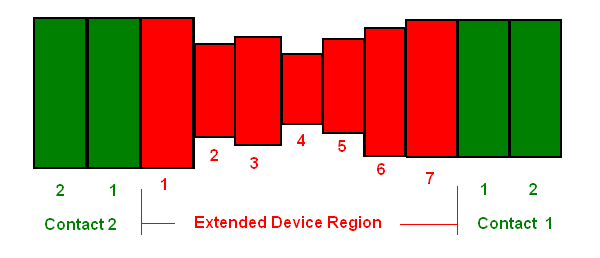
\includegraphics[width=0.8\linewidth]{layers.png}
\caption{Subdivision of a 2-terminal structure into principal layers (PL), two for each contact and an arbitrary number within the extended molecule.}
\label{layers}
\end{figure}

The extended molecule contains the atomistic device itself plus those parts of the attached electrodes, which are directly influenced by the presence of the device. Each electrode, on the other hand, contains those parts of the physical electrode, which are far enough from the device and are not affected by it. Examples below will better clarify this point.

The most important concept to bear in mind is that of principal layers (PLs). These are defined as contiguous groups of atoms that have interaction only with atoms of adjacent PLs. In practice these layers must contain a sufficient number of atoms in order to ensure that Hamiltonian and overlap interactions with second neighbouring PLs vanish or can be considered negligible. The subdivision into PLs is essential for the definition of the two contacts and becomes useful in the computation of all Green functions that exploit a recursive algorithm \cite{Pecchia08njp}.

As shown in the figure\,\ref{layers}, the extended molecule can contain an arbitrary number of PLs ($\geqslant 1$), but the layers must follow a sequential ordering.

{\bf The ordering of the PLs follows directly from the ordering of the atoms in the \dftbp structure.\footnote{Note, however, the case of model calculations without geometry Sec.\,\ref{sec-model}.}}

Typically it is convenient to create the structure and then sort the atom along the transport coordinate, before partitioning the system. In other cases, when nanowires are constructed it is convenient to repeat a PL unit for the desired length of the extended molecule.

The (perfect) contacts must be defined by two principal layers. Differently from the layers of the extended molecule, those defining the contacts must follow additional rules:
%
\begin{itemize}
\item The two principal layers of a given contact must be identical;
\item They must be rigidly shifted images of each other;
\item The first PL must be the closest to the device region.
\end{itemize}

In order to ensure the above prescriptions, the numbering of the atoms must follow a precise ordering.

The atoms of the central region must be specified first, before the atoms of the contacts (see example below in Fig.\,\ref{device_numbering}). The atoms of the contacts follow the central region. The atoms of each contact must be specified continously. (You specify either all atoms of the left contact first, and then those of the right one, or vice versa.)

The numbering inside the first principal layer defining each contact is arbitrary, but the same numbering must be applied to the second PL. Thus, the indices of the corresponding atoms in the two contact PLs must differ by the same value, and the coordinates must differ by the same translation vector. These prescriptions are checked by the code and an error message is issued if the two PLs do not conform. It is important to remember to place the first PL closer to the device, i.e. the principal layer closer to the device must contain the atoms with lower indices.

\begin{figure}[htbp]
\centering
\capstart
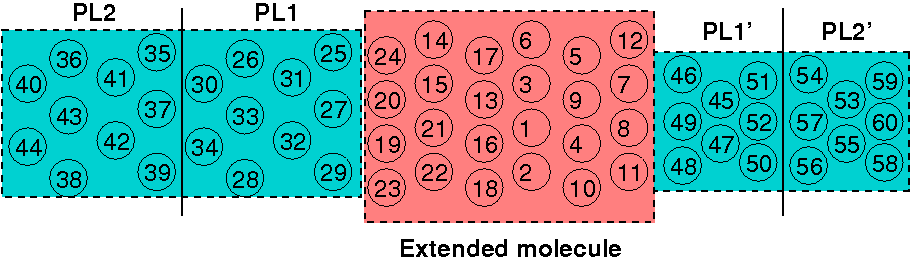
\includegraphics[width=0.8\linewidth]{device_numbering.png}
\caption{Example for numbering the atoms. Atoms of the device have the lowest indices, followed by the atoms of each contact, respectively. The two principal layers of both contacts are shifted images of each other.}
\label{device_numbering}
\end{figure}

\subsection{Supercell structures}

The code can compute transport on structures that have a periodicity in the transverse directions (with respect to transport). In this case the structure must be defined as a supercell and the rules listed above apply to each cell. The real-space Poisson solver of \dftbp limits the supercell lattices to orthorombic types (all angles between supercell vectors must be 90 degrees). In fact the supercell is always defined 3-dimensional, and the user should ensure that the dummy lattice vector along the transport direction is long enough to avoid superpositions between images.

The current version of \dftbp only supports one supercell definition for the entire system, including central region and contacts. It may be redundant to observe that in this case the two contacts must be of the same periodicity.

\subsection{Partitioning the system with N electrodes}

\dftbpxt allows also multi-terminal calculations. The rules for the atomic sequence are the same: first must be the device atoms, then the electrodes represented by two PLs each, and the numbers of the PL close to the device should be smaller than the numbers of the second PL.

In the case when the device region consists of many PLs, it is important that every electrode is connected to only one of PLs, but any number can be connected to one PL. The trivial example is the the case with only one PL in the central region and two electrodes, in this case both electrodes are connected to the same PL. This is illustrated in Fig.\,\ref{Nterminal}.

\begin{figure}[htbp]
\centering
\capstart
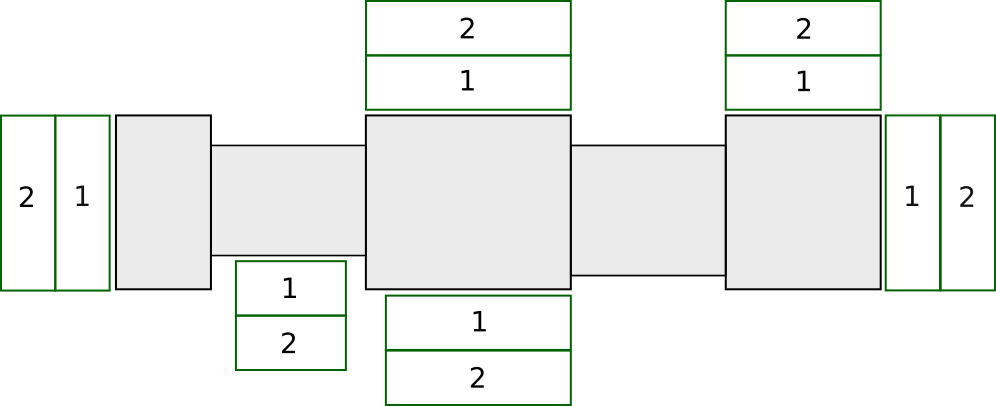
\includegraphics[width=0.8\linewidth]{Nterminal.png}
\caption{Subdivision of a N-terminal structure into principal layers (PL), two for each contact and an arbitrary number within the extended molecule.}
\label{Nterminal}
\end{figure}

\subsection{\is{Geometry} input block}

The atomic structure is defined in the \is{Geometry} block (see the \is{USER MANUAL} for the description). The example of geometry definition is given in the tutorial, see from Sec.\,\ref{electstruct:geometry-density-of-state}. 
  
\subsection{\is{Transport} input block}

The geometry must be additionally defined in the input \is{Transport} block as specified in the following example:

\begin{verbatim}
Transport {
   Device {
      AtomRange = 1 8
   }
   Contact {
      Id = "source"
      AtomRange = 9 24
      FermiLevel [eV] = -8.4123
      Potential = 0.0 
   }
   Contact {
      Id = "drain"
      AtomRange = 25 40
      FermiLevel [eV] = -8.4123
      Potential = 1.0 
   }
   Task = UploadContacts
}
\end{verbatim}

The Fermi level should be precalculated in the electrodes as discussed in Sec.\,\ref{sec-contacts} and in the tutorial in more detail. There are also many other parameters of the electrodes.

\section{Specifying the Hamiltonian}

\subsection{\is{Hamiltonian} input block}

The \is{Hamiltonian} block for Non-SCC DFTB calculations looks like

\begin{verbatim}
Hamiltonian = DFTB {
   SCC = No
   MaxAngularMomentum = {
      C = "p"
      H = "s"
   }
   SlaterKosterFiles = Type2FileNames {
      Prefix = "../../../sk/"  
      Separator = "-"
      Suffix = ".skf"
   }
   Eigensolver = TransportOnly{}
}
\end{verbatim}

Note that transport calculation can be started immediately in this case, but precalculations of electrodes may be done to determine the Fermi levels.

In the case of SCC DFTB calculation, however, the self-consistent density of electrons should be calculated at zero or finite voltage before the calculation of the transmission or density of states. The \is{Hamiltonian} block should include new options, the main are

\begin{verbatim}
Hamiltonian = DFTB {
   SCC = Yes
   SCCTolerance = 1e-6
   ReadInitialCharges = No 
   Electrostatics = Poisson {
      Poissonbox [Angstrom] = 40.0 30.0 30.0
      MinimalGrid [Angstrom] = 0.5 0.5 0.5
      SavePotential = Yes
   }
   Eigensolver = GreensFunction{}
   Mixer = Broyden{}
      MixingParameter = 0.02
   }
   ...
}  
\end{verbatim}

Note change of the \is{Eigensolver} method and new \is{Electrostatics} subblock, required for a self-consistent calculation of electron densities and electric field.

\subsection{Green function solver}

If you calculate electron transport properties using the Green function formalism, you need to determine the electron density in your system with respect to certain electrostatic boundary conditions for your system. For that, you must use the \iscb{GreensFunction} as eigensolver, which is capable to deliver the appropriate density. Please note, that this technique does not deliver any eigenvalues, it does not solve the eigenproblem (no eigenvectors are computed).

You can instruct the code to use the Green function solver by setting \is{Eigensolver} in the block \iscb{Hamiltonian = DFTB} to \iscb{GreensFunction}:

\begin{verbatim}
Hamiltonian = DFTB {
   :
   Eigensolver = GreensFunction{}
   :
}
\end{verbatim}

Let us discuss the most important parameters to be set in \iscb{GreensFunction}:

\begin{verbatim}
Eigensolver = GreensFunction {
   FirstLayerAtoms =  1   61   121   181   241   301   361   421   481   541
   Delta [eV] = 1e-4
   ContourPoints = 20 20
   LowestEnergy [eV] = -60.0
   EnclosedPoles = 0
}
\end{verbatim}

\is{FirstLayerAtoms}
is used to specify the PLs in the central region in the same way as described in \is{Device} subblock. Can be specified only if no  \is{Transport} block exists. As the name of the keyword suggests the layers are defined by specifying the first atom of each layer. In this case 10 PLs have been defined. Note that the contacts are not included here, as they are specified in the \is{Transport} block.

\is{Delta}
defines a small positive imaginary number used in the computation of the GFs.

\is{ContourPoints}
is used to specify the number of quadrature points in the contour integration (see also the \is{USER MANUAL} for a description of the complex contour).

\is{LowestEnergy}
is the initial energy from which the integration starts. It should be
low enough to ensure that all the electronic states are correctly included in the integration.
The default is -2.0 Hartree.

\is{EnclosedPoles}
    is set to 0 when T=0. For T>0 few poles (usually 3) needs to be included within the contour. 

\subsection{Poisson solver options}

For the transport calculation the \is{GammaFunctional} solver (default) is substituted with the \is{Poisson} solver. The \iscb{Poisson} method is used to define the size of the Poisson domain. The Poisson equation is solved via a real-space multigrid solver that employs finite-differences for discretization on a finite box with a regular grid (structured mesh). The charge density on the right-hand-side is constructed exactly as in standard gamma-functional of DFTB, namely expanding the charge density into spherical s-like atomic densities weighted by atomic Mulliken charges.

\begin{verbatim}
Electrostatics = Poisson {
   Poissonbox [Angstrom] = 30.0 30.0 30.0
   MinimalGrid [Angstrom] = 0.4 0.4 0.4
   AtomDensityTolerance = 1e-6
   BuildBulkPotential = Yes
   SavePotential = Yes
   PoissonAccuracy = 1e-7
}
\end{verbatim}

The method \iscb{Poisson} is used to define the size of the Poisson domain. The Poisson equation is solved via a real-space multigrid solver that employs finite-differences for discretization on a finite box with a regular grid (structured mesh). The charge density on the right-hand-side is constructed exactly as in standard gamma-functional of DFTB, namely expanding the charge density into spherical s-like atomic densities weighted by atomic Mulliken charges.

The equation is solved by imposing the following boundary conditions (BC):
\begin{enumerate}
\item Dirichelet or mixed BC on the faces containing contacts.
\item Neumann BC on the remaining faces. 
\end{enumerate} 

In the example above a box of 30x30 Angstrom in the $x$- and $y$- directions (orthogonal to the transport direction $z$) have been chosen. This size should be sufficient in the current case for obtaining a converged result. A box too small may introduce artificial size effects. The specification of the box length along the $z$-direction is a dummy number ignored by the code as the box-length in this direction is constrained by the position of the contacts and is internally adjusted.

The meaning of the additional options are the following:

\is{MinimalGrid = 0.4 0.4 0.4}
    is used to specify that the grid must be spaced less than 0.4 $\AA$ in all dimensions. The actual grid is adjusted internally since the number of grid points in every direction must be a power of 2 (exactly $N = 2^n + 1$).

\is{AtomDensityTolerance = 1e-6}
    is used to specify, where the exponential decaying spherical s-like atomic charge densities should be cut off. Specifying a certain value here makes sure that all atoms contributing a density higher than the given value are considered when calculating the amount of charges in a certain point (default: 1e-5). The appropriate cutoff radius is calculated automatically by the code (and reported in the output). It is determined by finding the cutoff distance for each atom ($\alpha$), where the s-like charge density
%
$$ n_\alpha(r) = \frac{\tau_{\alpha}^3}{8 \pi} e^{-\tau_{\alpha}r} $$
%
becomes smaller than the given tolerance. Then the maximal cutoff found for all atom types in the system is used. The quantity $\tau_{\alpha}= \frac{16}{5} U_{\alpha}$ is the relationship between the extintion coefficient and the Hubbard parameter in atomic units. See Ref.\,\cite{Elstner98prb}.

    In order to have a consistent calculation, the determined cutoff length must be smaller than the width of the principal layers when doing a calculation with contacts. The program will check for this criterion and stop if it is not fulfilled. In this example we set it exactly to the default value, only for clarification purpose. 
    
\is{CutoffCheck}
    If set to \is{No}, the code omits the check whether the cutoff for the atomic densities (either determined by \is{AtomDensityTolerance} or directly set by \is{AtomDensityCutoff}) is larger than the widths of the principal layers in the contacts. Please note that a cutoff bigger than the width of any contact PL results in inconsistent calculation, so it is highly discouraged to turn this check off, unless you exactly know what you are doing. (for experts only) 

\is{BuildBulkPotential = Yes}
    is used to specify that at the device/contact interfaces the bulk potential must be imposed as BC. The bulk potential is computed for an ideal contact (infinite wire). Here we should remind that a key assumption in transport calculations is that the contacts are in equilibrium and that the device/contact interfaces are sufficiently deep inside such that bulk conditions are recovered. This means that the charge density and potential at this interface should smoothly join with the bulk values. Setting this flag to Yes is important whenever there is a charge redistribution within the contact atoms that has an effect on the bulk potential, like in structures of heteronuclear species (e.g. SiC, GaAs, ZnO, etc.). In the case of a SiNW it is important because of the charge redistribution between silicon and hydrogen atoms.

    The bulk potential is computed by solving a Poisson problem for the contact PLs using a box with the same size and grid as specified for the central region along the $x$ and $y$ directions. In this way the result of the calculation is imposed on the device box without the need of interpolations.

    The problem is solved by imposing periodic boundary conditions (PBC) along the $z$-direction and Dirichelet BC on the other four sides (V=0). Note that this is not exactly consistent with the contact calculation performed on the first step, in which it was assumed a periodic structure with a large contact separation (1000 a.u.). However the two calculations produce approximately the same result. In principles the bulk potential could be computed exactly in the same way, by imposing a supercell with a large periodicity on the $(x,y)$ directions. The problem here is of technical nature because it is impractical to solve the Poisson equation on such a huge box (it would require a box with at least 1025x1025x257 grid points and a memory consumption of about 6.5 Gb). Secondly the Poisson equation generates a singular matrix when PBC are imposed on all sides of the box. A possibility (which is automatically switched on in supercells) is to compute the bulk potentials with an Ewald summation technique, but turns out to be quite time-consuming.

    In order to achieve better consistency with the contact calculations it is possible to compute the contact Hamiltonians using the Poisson solver rather than the usual \is{GammaFunctional}. This option can be set by specifying:
    
\is{Electrostatics = Poisson{}}

\dftbp recognizes if 1D wires are computed and imposes in this special case the same BC as in the bulk calculation, namely PBC along $z$ and Dirichelet on the other four sides. This procedure usually makes the equilibrium transmission function closer to the ideal conductance steps, since contact and device Hamiltonians are computed on an equal footing.

\subsection{Model calculations without geometry}
\label{sec-model}

Starting from the version {\textsf{DFTB$^{\text{+}}$XT 1.01}} the calculations with external model tight-binding Hamiltonians are possible. In particular ``without geometry'', it means that the coordinates are not used and are not required. It must be announced in the input file as

\begin{verbatim}
Geometry = NoGeometry{}
\end{verbatim}

In the \is{Transport} block it is only one important addition: \is{ContactPLs} describes the numbers of PLs to which the electrodes are coupled:

\begin{verbatim}
Transport {
   Device {
      AtomRange = 1 37
      FirstLayerAtoms =  1 9 19
      ContactPLs = 1 3            #Required for NoGeometry
   }
}
\end{verbatim}

Otherwise, it is described the geometry in the same way as before with the same assumptions about the order of tight-binding states (which are assumed to be ``atoms'' now). One atom corresponds to one electronic state. As a life hack, one can use the geometry from only hydrogen atoms (with only one electronic state) to create the real space tight-binding geometry, for example to include the self-consistent electric fields.

The \is{Analysis} block is also unchanged.

Most important is the change in the \is{Hamiltonian} block. It looks like

\begin{verbatim}
Hamiltonian = Model { 
   NumStates = 44                   #Required for NoGeometry 
   HamiltonianFile [eV] = H.mtr   #Relevant for NoGeometry (default is H.mtr, [eV])
   SpinDegeneracy = Yes            #Relevant for NoGeometry 
}  
\end{verbatim}

The new method is \iscb{Model}, it includes the required parameter \is{NumStates}, which gives the full number of states including the central region and the electrodes. The \is{HamiltonianFile} can be used to change the name of the Hamiltonian and the energy units. Finally, \is{SpinDegeneracy = Yes} says that there are two electrons in every state (just to multiply the DOS and transmission by 2).

The Hamiltonian \is{H.mtr} should be saved as an array of real numbers. It should be ordered in the right way corresponding to the numbering of sites and be consistent with the ordering of sites (atoms) in the \is{Transport} block!

{\bf The ordering of the PLs and sites in PLs follows directly from the ordering of the states in the external Hamiltonian.}

At the moment users should care about the right ordering.


\section{Precalculation of electrodes}
\label{sec-contacts}

A transport calculation requires the execution of preliminary tasks for the computation of the contact Hamiltonians. The contacts are assumed ideal and having the properties of a ‘bulk’ material. For this reason a special calculation must be performed in advance and results are stored on files for subsequent uploading.

The \is{Transport} block contains a \is{Task} block, which describes the action to be carried out. The following tasks can be executed:

\iscb{Task = UploadContacts}

for transport calculations, or

\iscb{Task = ContactHamiltonian}

to calculate the Hamiltonian for a given contact. The name of the contact must be specified via the \is{Id} tag. Only one contact Hamiltonian can be calculated at one go, so that you have to run \dftbp for every contact separately.

The example below demonstrates the contact calculation for the contact called “source”:

\begin{verbatim}    
    Transport {
      Device {
        AtomRange = 1 24
      }
      Contact {
        Id = "source"
        AtomRange = 25 44
      }
      Contact {
        Id = "drain"
        AtomRange = 45 58
      }
      Task = ContactHamiltonian {
        ContactId = "source"
      }
    }
\end{verbatim} 

\section{Calculation of transmission and density of states}

Using the electrode Hamiltonians produced with \iscb{Task = ContactHamiltonian}, the surface Green functions for the contacts can be calculated, and open boundary conditions are applied. To calculate the electronic transport through the device, defined in \is{Geometry}, \is{Transport} and \is{Hamiltonian} blocks, one should define the additional parameters in the \is{Analysis} block.

\subsection{\is{Analysis} input block}

In the simplest case it looks like 
%
\begin{verbatim} 
Analysis{
   TunnelingAndDOS{
      EnergyRange [eV] = -5.0 -3.0
      EnergyStep [eV] = 0.02
      Region = {
         Atoms = 1:37
      }
   }
}
\end{verbatim}

\is{EnergyRange} and \is{EnergyStep} determine the energy range over which the transmission function and local
density of states are computed and the energy step.

\is{Region} defines atomic ranges or orbitals where the local density of states is calculated projected. The definition in the block follow the same syntax as a \dftbp calculation without transport.

See the \is{USER MANUAL} for details. The examples of transport calculations are given in the tutorial, see   {\hyperref[transport:electron-transport-calculations-in-armchair-nanoribbons]{Chapter\,\ref{transport:electron-transport-calculations-in-armchair-nanoribbons} Electron transport calculations in armchair nanoribbons}.

\part{Tutorial on 2D Carbon Materials}
\label{2Dtutorial}    

\chapter{Introduction}
\label{introduction:dftb-tutorial-on-2d-carbon-materials}\label{introduction:introduction}\label{introduction::doc}
This tutorial is aimed at Master and PhD students with
background knowledge of the theory of electronic structure and quantum
transport at nanoscale. Minimal knowledge of Unix/Linux is also
required. Knowledge of the \dftbpxt code itself is not necessary, but
familiarity with the basic ideas behind the Density Functional Theory (DFT), the Density Functional Tight
Binding (DFTB) method, the Landauer method and the Green function technique of the quantum transport theory could be helpful.


\section{System environment}
\label{introduction:system-environment}
The easiest way to use this tutorial is to download the {\textsf{DFTB$^{\text{+}}$XT LiveDVD}} ISO
image from the \href{http://quantranspro.org/dftb+xt/}{quantranspro.org/dftb+xt/} site, which contains a preconfigured x86\_64/Linux system with all the
necessary tools for the tutorial. One can directly boot the ISO image
within a virtual machine (e.g. \emph{VirtualBox}). Alternatively, one can
create a bootable USB-drive (e.g. with \emph{usb-creator} under Linux or
\emph{Universal USB Installer} under Windows) or DVD, which can then be
used to boot up an X86\_64 machine with the live system.

In case you want to try the tutorial outside of the live system, you
will need the following tools to be installed:

\begin{itemize}
  
\item {} 
\emph{dftb+} -- \dftbpxt binary (version 1.01 or higher).

\item {} 
\emph{waveplot} -- Command line tool to create volumetric data files
representing electron densities and wavefunctions. (included into the \dftbpxt package and is installed together with \emph{dftb+}) 

\item {} 
\emph{nano} -- A simple graphical text editor. You can alternatively
use your preferred editor instead.

\item {} 
\emph{gen2xyz}, \emph{xyz2gen}, \emph{dp\_dos}, \emph{dp\_bands}, \emph{repeatgen}, \emph{makecube} -- Various conversion scripts from
the \emph{dp\_tools} package. (included into the \dftbpxt package, but should be installed separately)

\item {} 
\emph{jmol} -- Graphical molecular visualisation tool. You can
alternatively use any molecular visualiser able to plot volumetric
data and isosurfaces.

\item {} 
\emph{buildwire} -- Can be used to build a 1D geometry with the right ordering (included into the \dftbpxt package, but should be installed separately).

\item {} 
\emph{paraview} -- Software to visualise \emph{.vtk} or \emph{.cube} files.

\item {} 
\emph{plotxy[.py]} -- Command line wrapper around the matplotlib python library (included into the \dftbpxt package).  

\end{itemize}


\section{General notes}
\label{introduction:general-notes}\begin{itemize}
\item {} 
The working directory of each of the tutorial examples is indicated
at the beginning of its corresponding section. Please change to that
directory and execute the specified commands from within that
directory.

\item {} 
It is impossible to describe all options accepted by \dftbpxt within
the tutorial. The detailed description of input and output is given in the \is{USER MANUAL}.
Always make sure, that you understand the input file
for \dftbp (\emph{dftb\_in.hsd}). If you find any unexplained options,
consult the \href{http://quantranspro.org/dftb+xt/documentation.html}{\dftbpxt documentation page} and the \href{http://www.dftb-plus.info/documentation/}{\dftbp documentation page} for details.

\item {} 
In order to save you some typing, many of the necessary commands
have been already collected into small scripts. Please have a look
at the content of these scripts before executing them, making sure
you understand why those commands must be executed in that order to
obtain the necessary results.

\item {} 
The {\textsf{DFTB$^{\text{+}}$XT LiveDVD}} version of the \dftbpxt code is free for use and full functional.
It can be used to install the standard Debian GNU/Linux operating system.

\end{itemize}

\section{Creating of the directory with inputs}

Please download the file \emph{tutorial\_input.zip} from the \dftbpxt site or copy it from the \emph{/doc/dftb+/tutorial/} folder of the package. Then decompress it with:
%
\begin{Verbatim}[commandchars=\\\{\}]
unzip tutorial\_input.zip
\end{Verbatim}

in some directory. The directory tree with input files and some additional files to speed up the calculations is created.

\null
If use the {\textsf{DFTB$^{\text{+}}$XT LiveDVD}}, the tree with input files is placed in \emph{/home/user/Tutorial}, where one can also find the \emph{guide.pdf} and \emph{manual.pdf} files.

\null
Note, that if you first install the Debian GNU/Linux from LiveDVD to the hard disk, the tutorial materials will be still in \emph{/home/user/Tutorial} and you should use the root access to copy it to your actual home directory and change access rights. The same should be done for \emph{/home/user/bin} with executable files and, finally, \emph{export PATH=\$PATH:\$HOME/bin} to make short commands available.

\chapter{Electronic structure of 2D carbon materials}
\label{electstruct:electronic-structure-of-2d-carbon-materials}\label{electstruct::doc}

Enter the directory \emph{elect/}. All
directories given in this part of the tutorial are subdirectories of
the \emph{elect/} directory.


\section{Perfect graphene}
\label{electstruct:perfect-graphene}
First we will investigate some of the basic properties of the 2D
graphene structure.


\subsection{Geometry, density of state}
\label{electstruct:geometry-density-of-state}
{[}Working directory: \emph{elect/graphene/latopt/}{]}


\subsubsection{Preparing the input}
\label{electstruct:preparing-the-input}
Graphene has a hexagonal lattice with two C atoms in its primitive
unit cell, which is specified in the supplied GEN-formatted geometry
file. Open the file \emph{geo.gen} in a text editor

\begin{Verbatim}[commandchars=\\\{\}]
nano geo.gen
\end{Verbatim}

You should see the following content:

\begin{Verbatim}[commandchars=\\\{\}]
2  S
C
 1 1    0.1427557522E+01    0.0000000000E\PYGZhy{}00    0.0000000000E\PYGZhy{}00
 2 1   \PYGZhy{}0.1427557522E+01    0.0000000000E\PYGZhy{}00    0.0000000000E\PYGZhy{}00
 0.0000000000E+00    0.0000000000E+00    0.0000000000E+00
 0.2141036415E+01   \PYGZhy{}0.1236340643E+01    0.0000000000E\PYGZhy{}00
 0.2141036415E+01    0.1236340643E+01    0.0000000000E\PYGZhy{}00
 0.0000000000E\PYGZhy{}00    0.0000000000E\PYGZhy{}00    0.5000000000E+02
\end{Verbatim}

The format of this GEN file is the following:
\begin{itemize}
\item {} 
The first line contains the number of atoms (\code{2}) and the boundary
condition type (\code{S} for a periodic crystal).

\item {} 
The second line lists all atomic elements present in the system
separated by white space (\code{C} only in this example).

\item {} 
Then a squence of lines follow, one for every atom in the system,
each starting with a dummy integer (its sequential number in the
structure), the type of the atom according to the list of elements
in the second line of the file (\code{1} for carbon in this example),
and finally the cartesian coordinates of the atom in angstroms.

\item {} 
Since the structure is periodic, appropriate information for this
boundary condition must be provided after the atomic
coordinates. For a GEN file of type \code{S}, this is the cartesian
coordinates of the origin followed by the 3 cartesian lattice
vectors (one per line). \dftbp uses three dimensional periodic
boundary conditions. In order to separate the graphene sheets from
each other and to prevent interaction between them, the third
lattice vector, which is orthogonal to the plane of graphene, has
been chosen to have a length of 50 angstroms.

\end{itemize}

Before running the code, you should check, whether the specified unit
cell, when repeated along the lattice vectors, indeed results in a
proper graphene structure. To repeat the geometry along the first and
second lattice vectors a few times (the \emph{repeatgen} script), convert
it to XYZ-format (the \emph{gen2xyz} script) and visualize it:

\begin{Verbatim}[commandchars=\\\{\}]
repeatgen geo.gen 4 4 1 \PYGZgt{} geo.441.gen
gen2xyz geo.441.gen
jmol geo.441.xyz \PYGZam{}
\end{Verbatim}

You should then see a graphene sheet displayed, similar to Figure
{\hyperref[electstruct:fig-graphene-441]{\emph{\DUspan{}{4x4x1 graphene supercell}}}} (\autopageref*{electstruct:fig-graphene-441}).
\begin{quote}
\begin{figure}[htbp]
\centering
\capstart
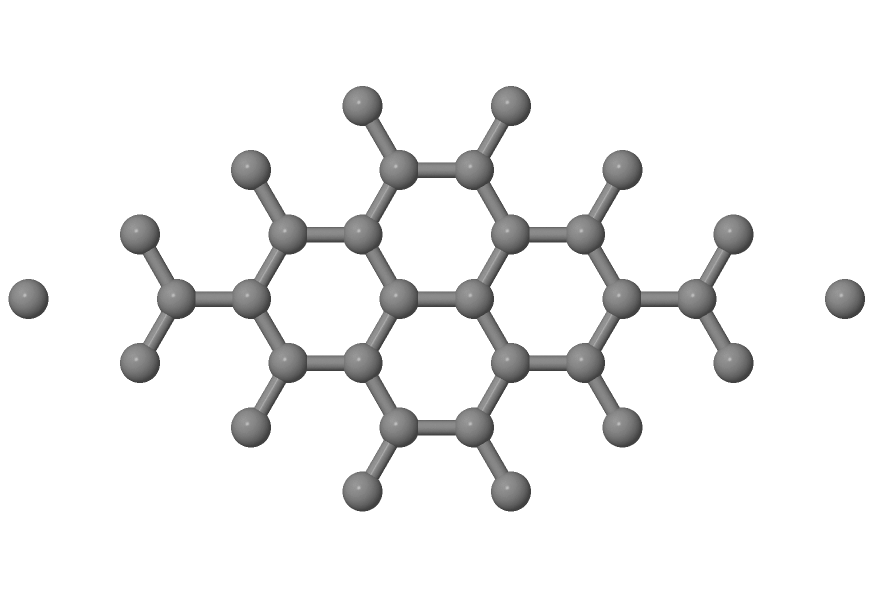
\includegraphics[width=0.600\linewidth]{geo-441.png}
\caption{4x4x1 graphene supercell}\label{electstruct:fig-graphene-441}\end{figure}
\end{quote}

Now open the \dftbp control file \emph{dftb\_in.hsd}.

\begin{Verbatim}[commandchars=\\\{\}]
nano dftb\PYGZus{}in.hsd
\end{Verbatim}

You should see the following options within it:
\begin{itemize}
\item {} 
First we include the GEN-formatted geometry file, \emph{geo.gen}, using
the inclusion operator (\code{\textless{}\textless{}\textless{}}):

\begin{Verbatim}[commandchars=\\\{\}]
Geometry = GenFormat \PYGZob{}
   \PYGZlt{}\PYGZlt{}\PYGZlt{} \PYGZdq{}geo.gen\PYGZdq{}
\PYGZcb{}
\end{Verbatim}

\item {} 
Then we specify the \code{ConjugateGradient} driver to optimize the
geometry and also the lattice vectors. Since neither the angle
between the lattice vectors nor their relative lengths should change
during optimization, we carry out an isotropic lattice
optimization:

\begin{Verbatim}[commandchars=\\\{\}]
Driver = ConjugateGradient \PYGZob{}
  LatticeOpt = Yes
  Isotropic = Yes
\PYGZcb{}
\end{Verbatim}

\item {} 
Then the details of the DFTB hamiltonian follow:

\begin{Verbatim}[commandchars=\\\{\}]
Hamiltonian = DFTB \PYGZob{}
\end{Verbatim}

\item {} 
Within this block, we first specify the location of the
parametrization files (the Slater-Koster files) and provide
additional information about the highest angular momentum for each
element (this information is not yet stored in the
Slater-Koster-files):

\begin{Verbatim}[commandchars=\\\{\}]
MaxAngularMomentum \PYGZob{}
  C = \PYGZdq{}p\PYGZdq{}
\PYGZcb{}
SlaterKosterFiles = Type2FileNames \PYGZob{}
  Prefix = \PYGZdq{}../../../sk/\PYGZdq{}
  Separator = \PYGZdq{}\PYGZhy{}\PYGZdq{}
  Suffix = \PYGZdq{}.skf\PYGZdq{}
\PYGZcb{}
\end{Verbatim}

Please note, that the highest angular momentum is \textbf{not a free
parameter} to be changed, but it must correspond to the value given
in the documentation section of the correspoding homonuclear
Slater-Koster-files (e.g. see the \emph{C-C.skf} file for carbon).

\item {} 
We use the self-consistent charge approach (SCC-DFTB), enabling
charge transfer between the atoms:

\begin{Verbatim}[commandchars=\\\{\}]
\PYG{n}{SCC} \PYG{o}{=} \PYG{n}{Yes}
\end{Verbatim}

\item {} 
As graphene is metallic we smear the filling function to achieve better
SCC-convergence:

\begin{Verbatim}[commandchars=\\\{\}]
Filling = Fermi \PYGZob{}
  Temperature [Kelvin] = 100
\PYGZcb{}
\end{Verbatim}

\item {} 
For the Brillouin-zone sampling we set our k-points according to the
48 x 48 x 1 Monkhorst-Pack sampling scheme. This contains those
k-points which would be folded onto the k-point (0.5, 0.5, 0.0) of
an enlarged supercell consisting of the primitive unit cell repeated
by (48, 0, 0), (0, 48, 0) and (0, 0, 1). This can be easily
specified with the \code{SupercellFolding} option, where one defines
those supercell vectors followed by the target k-point.

\begin{Verbatim}[commandchars=\\\{\}]
KPointsAndWeights = SuperCellFolding \PYGZob{}
  48 0 0
  0 48 0
  0 0 1
  0.5 0.5 0.0
\PYGZcb{}
\end{Verbatim}

\item {} 
We also want to do some additional analysis by evaluating the
contributions of the \emph{s}- and \emph{p}-shells to the density of states
(DOS). Accordingly, we instruct \dftbp in the \code{Analysis} block to
calculate the contribution of all C atoms to the DOS in a shell-wise
manner (s and p) and store the shell-contributions in files starting
with a prefix of \emph{pdos.C}:

\begin{Verbatim}[commandchars=\\\{\}]
Analysis \PYGZob{}
  ProjectStates \PYGZob{}
    Region \PYGZob{}
      Atoms = C
      ShellResolved = Yes
      Label = \PYGZdq{}pdos.C\PYGZdq{}
    \PYGZcb{}
  \PYGZcb{}
\PYGZcb{}
\end{Verbatim}

\end{itemize}


\subsubsection{Running the code}
\label{electstruct:running-the-code}
When you run \dftbp, you should always save its output into a file for
later inspection. We suggest using a construction like this (output is
saved into the file \emph{output}):

\begin{Verbatim}[commandchars=\\\{\}]
dftb+ \textbar{} tee output
\end{Verbatim}

You will see that \dftbp optimizies the geometry of graphene by
changing the lattice vectors and ion coordinates to locally minimise
the total energy. As the starting geometry is quite close to the
optimum one, the calculation should finish almost immediately.

Apart from the saved output file (\emph{output}), you will find several
other new files created by the code:
\begin{description}
\item[{\emph{dftb\_pin.hsd} Contains the parsed user input with all the default}] \leavevmode
settings for options which have not been explicitely set by the
user. You should have look at it if you are unsure whether the
defaults \dftbp used for your calculation are appropriate, or if you
want to know which other options you can use to adjust your
calculation.

\item[{\emph{detailed.out} Contains detailed information about the calculated}] \leavevmode
physical quantities (energies, forces, eigenlevels, fillings,
charges, etc.)  obtained in the last SCC cycle performed.

\item[{\emph{band.out} Eigenvalues (in eV) and fillings for each k-point and spin}] \leavevmode
channel.

\item[{\emph{charges.bin} Charges of the atoms at the last iteration, stored in}] \leavevmode
binary format. You can use this file to restart a calculation with
those atomic charges.

\item[{\emph{geo\_end.xyz}, \emph{geo\_end.gen} Final geometry in both XYZ and GEN}] \leavevmode
formats.

\item[{\emph{pdos.C.1.out}, \emph{pdos.C.2.out} Output files containing the projected}] \leavevmode
density of states for the first and second angular shells of carbon
(in this case the \emph{2s} and \emph{2p} shells). Their format is similar to
\emph{band.out}.

\end{description}


\subsubsection{Analysing results}
\label{electstruct:analysing-results}
The very first thing you should check is whether your calculation has
converged at all to a relaxed geometry. The last line of the \emph{output}
file contains the appropriate message:

\begin{Verbatim}[commandchars=\\\{\}]
Geometry converged
\end{Verbatim}

This means that the program stopped because the forces on the atoms
which are allowed to move (all of them in this example) were less than
a given tolerance (specified in the option \code{MaxForceComponent},
which defaults to 1e-4 atomic units) and not instead because the
maximal number of geometry optimization steps have been executed
(option \code{MaxSteps}, default 200).

You should visualize the resulting structure using Jmol (or any other
molecular visualization tool). You should probably repeat the geometry
again to get a better idea how it looks like, as we did for the
starting structure above. The distance between the C atoms should be
very similar to those in the initial structure.

In order to visualize the density of states and the partial density of
states, you should convert the corresponding human readable files
(with prefix \emph{.out}) to XY-format data

\begin{Verbatim}[commandchars=\\\{\}]
dp\PYGZus{}dos band.out dos.dat
dp\PYGZus{}dos \PYGZhy{}w pdos.C.1.out pdos.C.1.dat
dp\PYGZus{}dos \PYGZhy{}w pdos.C.2.out pdos.C.2.dat
\end{Verbatim}

Please note the flag \code{-w}, which is mandatory when converting
\emph{partial} density of states data for plotting. You can obtain more
information about various flags for dp\_dos by issuing:

\begin{Verbatim}[commandchars=\\\{\}]
\PYG{n}{dp\PYGZus{}dos} \PYG{o}{\PYGZhy{}}\PYG{n}{h}
\end{Verbatim}

You can visualize the DOS and the PDOS for the \emph{s}- and \emph{p}-shells of
carbon in one picture using the \emph{plotxy} tool, which is a simple
command line wrapper around the matplotlib python library (issue the
command \code{plotxy -h} for help):

\begin{Verbatim}[commandchars=\\\{\}]
plotxy \PYGZhy{}\PYGZhy{}xlabel \PYGZdq{}Energy [eV]\PYGZdq{} \PYGZhy{}\PYGZhy{}ylabel \PYGZdq{}DOS\PYGZdq{} dos.dat pdos.C.1.dat pdos.C.2.dat \PYGZam{}
\end{Verbatim}

You can use also any other program (gnuplot, xmgrace) which can visualize
XY-data. You should see something similar to Figure {\hyperref[electstruct:fig-graphene-dos]{\emph{\DUspan{}{DOS and PDOS of graphene}}}} (\autopageref*{electstruct:fig-graphene-dos}).
% \begin{quote}
\vskip -0.2cm
\begin{figure}[htbp]
\centering
\capstart
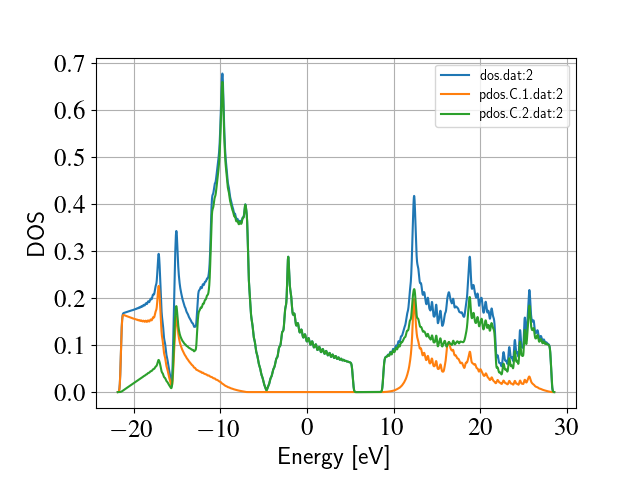
\includegraphics[width=0.650\linewidth]{graphene-dos.png}
\caption{DOS and PDOS of graphene}\label{electstruct:fig-graphene-dos}\end{figure}
%\end{quote}

The position of the Fermi level (at -4.67 eV) can be read out from the
\emph{detailed.out} file, either directly or by using an appropriate \emph{grep}
command:

\begin{Verbatim}[commandchars=\\\{\}]
grep \PYGZdq{}Fermi level\PYGZdq{} detailed.out
\end{Verbatim}

As expected for graphene, the DOS vanishes at the Fermi-level. Around
the Fermi-level, all states are composed of the \emph{p}-orbitals of the
carbons, the \emph{s}-orbitals only contribute to energeticaly much lower
and much higher states. Also, one can observe the
van-Hove-singularties. The \code{wiggles} at around 0 eV and at higher
energy are artifacts. Using more k-points for the Brillouin-zone
sampling or using a slightly wider broadening function in \emph{dp\_dos}
would smooth them out.


\subsection{Band structure}
\label{electstruct:band-structure}
{[}Working directory: \emph{elect/graphene/bands/}{]}

Band structure calculations in DFTB (as in DFT) always consist of two
steps:
\begin{enumerate}
\item {} 
Calculating an accurate ground state charge density by using a high
quality k-point sampling.

\item {} 
Determining the eigenvalues at the desired k-points of the band
structure, using the density obtained in the previous step. The
density is not changed during this step of the band structure
calculation.

\end{enumerate}

Step 1 you just have executed, so you can copy the final geometry and the data
file containing the converged charges from that calculation into your current
working directory:

\begin{Verbatim}[commandchars=\\\{\}]
cp ../latopt/geo\PYGZus{}end.gen .
cp ../latopt/charges.bin .
\end{Verbatim}

Have a look on the \emph{dftb\_in.hsd} file for the band structure
calculation. It differs from the previous one only in a few aspects:
\begin{itemize}
\item {} 
We use the end geometry of the previous calculation as geometry:

\begin{Verbatim}[commandchars=\\\{\}]
Geometry = GenFormat \PYGZob{}
  \PYGZlt{}\PYGZlt{}\PYGZlt{} \PYGZdq{}geo\PYGZus{}end.gen\PYGZdq{}
\PYGZcb{}
\end{Verbatim}

\item {} 
We need static calculation only (no atoms should be moved),
therefore, no driver block has been specified.

\item {} 
The k-points are specified along specific high symmetry lines of the
Brillouin-zone (K-Gamma-M-K):

\begin{Verbatim}[commandchars=\\\{\}]
KPointsAndWeights = KLines \PYGZob{}
  1    0.33333333  0.66666666 0.0    \PYGZsh{} K
 20    0.0  0.0  0.0                 \PYGZsh{} Gamma
 20    0.5  0.0  0.0                 \PYGZsh{} M
 10    0.33333333  0.66666666 0.0    \PYGZsh{} K
\PYGZcb{}
\end{Verbatim}

\item {} 
We initialize the calculation with the charges stored during the
previous run:

\begin{Verbatim}[commandchars=\\\{\}]
\PYG{n}{ReadInitialCharges} \PYG{o}{=} \PYG{n}{Yes}
\end{Verbatim}

\item {} 
We do not want to change the charges during the calculation,
therefore, we set the maximum number of SCC cycles to one:

\begin{Verbatim}[commandchars=\\\{\}]
\PYG{n}{MaxSCCIterations} \PYG{o}{=} \PYG{l+m+mi}{1}
\end{Verbatim}

\end{itemize}

Let's run the code and convert the band structure output to
XY-format:

\begin{Verbatim}[commandchars=\\\{\}]
dftb+ \textbar{} tee output
dp\PYGZus{}bands band.out band
\end{Verbatim}

The dp\_bands tool extracts the band structure from the file \emph{band.out}
and stores it in the file \emph{band\_tot.dat}. For spin polarized systems,
the name of the output file would be different. Use:

\begin{Verbatim}[commandchars=\\\{\}]
\PYG{n}{dp\PYGZus{}bands} \PYG{o}{\PYGZhy{}}\PYG{n}{h}
\end{Verbatim}

to get help information about the arguments and the possible options
for dp\_bands.

In order to investigate the band structure we first look up the
position of the Fermi level in the previous calculation performed with
the accurate k-sampling

\begin{Verbatim}[commandchars=\\\{\}]
grep \PYGZdq{}Fermi level\PYGZdq{} ../latopt/detailed.out
\end{Verbatim}

which yields -4.67 eV, and then visualize the band structure by
invoking

\begin{Verbatim}[commandchars=\\\{\}]
plotxy \PYGZhy{}L \PYGZhy{}\PYGZhy{}xlabel \PYGZdq{}K points\PYGZdq{} \PYGZhy{}\PYGZhy{}ylabel \PYGZdq{}Energy [eV]\PYGZdq{} band\PYGZus{}tot.dat \PYGZam{}
\end{Verbatim}

This results in the band structure as shown in Figure
{\hyperref[electstruct:fig-graphene-band]{\emph{\DUspan{}{Band structure of graphene}}}} (\autopageref*{electstruct:fig-graphene-band}).
\begin{quote}
\begin{figure}[htbp]
\centering
\capstart

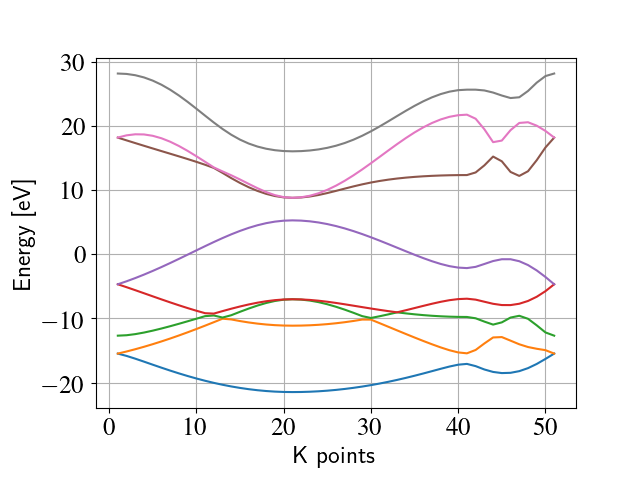
\includegraphics[width=0.650\linewidth]{graphene-band.png}
\caption{Band structure of graphene}\label{electstruct:fig-graphene-band}\end{figure}
\end{quote}

You can see the linear dispersion relations around the point \emph{K} in
the Brillouin-zone (k-points 0 and 51 in our circuit) which is a very
typical characteristic of graphene.


\section{Zigzag nanoribbon}
\label{electstruct:zigzag-nanoribbon}
Next we will study some properties of a hydrogen saturated carbon
zigzag nanoribbon.


\subsection{Calculting the density and DOS}
\label{electstruct:calculting-the-density-and-dos}
{[}Working directory: \emph{elect/zigzag/density/}{]}

The initial geometry for the zigzag nanoribbon contains one chain of
the structure, repeated periodically along the z-direction. The
lattice vectors orthogonal to the periodicity (along the x- and y-
axis) are set to be long enough to avoid any interaction between the
repeated images.

First convert the GEN-file to XYZ-format and visualize it:

\begin{Verbatim}[commandchars=\\\{\}]
gen2xyz geo.gen
jmol geo.xyz \PYGZam{}
\end{Verbatim}

Similar to the case of perfect graphene, you should check first the
initial geometry by repeating it along the periodic axis (the third
lattice vector in this example) and visualize it. The necessary steps
are collected in the file \emph{checkgeo.sh}. Please have a look at its
content to understand what will happen, and then issue

\begin{Verbatim}[commandchars=\\\{\}]
sh checkgeo.sh
\end{Verbatim}

to obtain the molecule shown in Figure {\hyperref[electstruct:fig-zigzag-114]{\emph{\DUspan{}{Section of an H-saturated zigzag nanoribbon}}}} (\autopageref*{electstruct:fig-zigzag-114}).
\begin{quote}
\begin{figure}[htbp]
\centering
\capstart

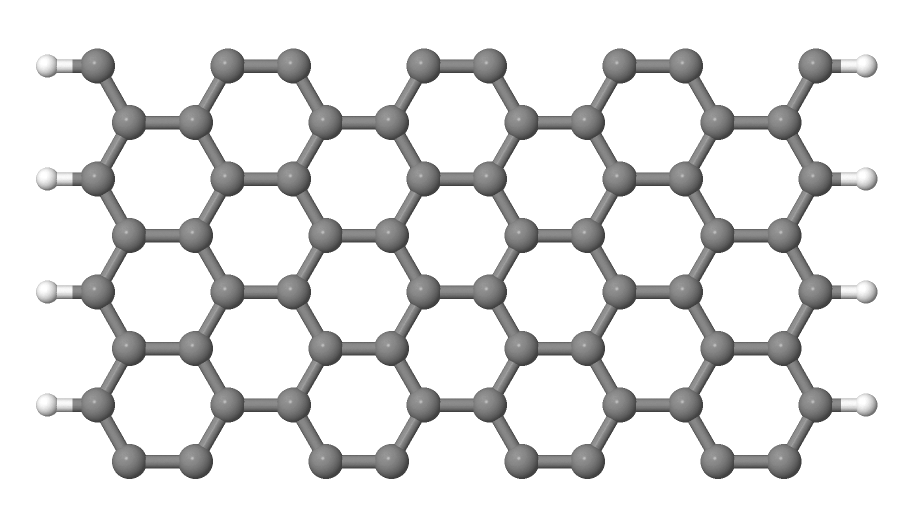
\includegraphics[width=0.600\linewidth]{geo-zigzag-114.png}
\caption{Section of an H-saturated zigzag nanoribbon}\label{electstruct:fig-zigzag-114}\end{figure}
\end{quote}

The control file \emph{dftb\_in.hsd} is similar to the previous examples,
with a few differences only:
\begin{itemize}
\item {} 
We use the 1 x 1 x 24 Monkhorst-Pack k-point set to sample the
Brillouin-zone, since the ribbon is only periodic along the
direction of the third lattice vector. The two other lattice vectors
have been choosen to be long enough to avoid interaction between the
artificially repeated ribons.:

\begin{Verbatim}[commandchars=\\\{\}]
KPointsAndWeights = SupercellFolding \PYGZob{}
  1 0 0
  0 1 0
  0 0 24
  0.0 0.0 0.5
\PYGZcb{}
\end{Verbatim}

\item {} 
In order to analyze, which atoms contribute to the states around the
Fermi-level, we create four projection regions containing the
saturating H-atoms, the C atoms in the outermost layer of the
ribbon, the C atoms in the second outermost layer and finally the C
atoms in the thirds outermost layer, respectively. Since the ribbon
is mirror symmetric, we include the corresponding atoms on both
sides in each projection region:

\begin{Verbatim}[commandchars=\\\{\}]
ProjectStates \PYGZob{}

  \PYGZsh{} The terminating H atoms on the ribbon edges
  Region \PYGZob{}
    Atoms = H
    Label = \PYGZdq{}pdos.H\PYGZdq{}
  \PYGZcb{}

  \PYGZsh{} The surface C atoms
  Region \PYGZob{}
    Atoms  = 2 17
    Label = \PYGZdq{}pdos.C1\PYGZdq{}
  \PYGZcb{}

  \PYGZsh{} The next row of C atoms further inside
  Region \PYGZob{}
    Atoms = 3 16
    Label = \PYGZdq{}pdos.C2\PYGZdq{}
  \PYGZcb{}

  \PYGZsh{} Some more \PYGZsq{}bulk\PYGZhy{}like\PYGZsq{} C atoms even deeper
  Region \PYGZob{}
    Atoms = 4 15
    Label = \PYGZdq{}pdos.C3\PYGZdq{}
  \PYGZcb{}
\PYGZcb{}
\end{Verbatim}

\end{itemize}

You can run the program and convert the output files by issuing:

\begin{Verbatim}[commandchars=\\\{\}]
sh run.sh
\end{Verbatim}

When the program has finished, look up the Fermi-level and visualize
the DOS and PDOS contributions. The necessary commands are collected
in \emph{showdos.sh}:

\begin{Verbatim}[commandchars=\\\{\}]
sh showdos.sh
\end{Verbatim}

When you zoom into the area around the Fermi level (-4.57 eV), you
should obtain something like Figure {\hyperref[electstruct:fig-zigzag-dos]{\emph{\DUspan{}{DOS of the zigzag nanoribbon around the Fermi energy}}}} (\autopageref*{electstruct:fig-zigzag-dos}).
\begin{quote}
\vskip -0.2cm  
\begin{figure}[htbp]
\centering
\capstart
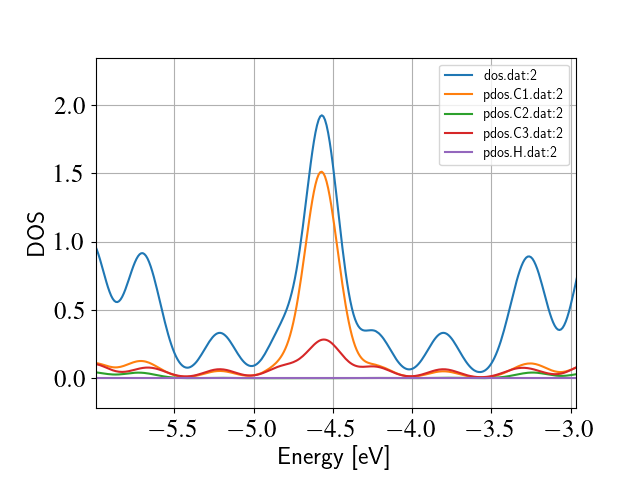
\includegraphics[width=0.650\linewidth]{zigzag-dos.png}
\caption{DOS of the zigzag nanoribbon around the Fermi energy}\label{electstruct:fig-zigzag-dos}\end{figure}
\end{quote}

You can see that the structure is clearly metallic (displaying a
non-zero density of states at the Fermi energy). The states around the
Fermi-level are composed of the orbitals of the C atoms in the
outermost and the third outermost layer of the ribbon. There is no
contribution from the C atom in the layer in between or from the H
atoms to the Fermi level.


\subsection{Band structure}
\label{electstruct:id1}
{[}Working directory: \emph{elect/zigzag/bands/}{]}

Now let's calculate the band structure of the zigzag nanoribbon. The
commands are in the script \emph{run.sh}, so just issue:

\begin{Verbatim}[commandchars=\\\{\}]
sh run.sh
\end{Verbatim}

You will see \dftbp finishing with an error message

\begin{Verbatim}[commandchars=\\\{\}]
WARNING!
\PYGZhy{}\PYGZgt{} SCC is NOT converged, maximal SCC iterations exceeded
\end{Verbatim}

Normally, it would mean that \dftbp did not manage to find a self
consistent charge distribution for its last geometry. In our case,
however, it is not an error, but the desired behaviour. We have
specified in \emph{dftb\_in.hsd} the options

\begin{Verbatim}[commandchars=\\\{\}]
\PYG{n}{ReadInitialCharges} \PYG{o}{=} \PYG{n}{Yes}
\PYG{n}{MaxSCCIterations} \PYG{o}{=} \PYG{l+m+mi}{1}
\end{Verbatim}

requiring the program to stop after one SCC iteration. The charges are
at this point not self consistent with respect to the k-point set used
for sampling the band structure calculation. However, k-points along
high symmetry lines of the Brillouin-zone, as used to obtain the band
structures, usually represent a poor sampling. Therefore the a
converged density obtained with an accurate k-sampling should be used
to obtain the eigenlevels, and no self consistency is needed.

To look up the Fermi-level and plot the band structure use the
commands in \emph{showbands.sh}:

\begin{Verbatim}[commandchars=\\\{\}]
sh showbands.sh
\end{Verbatim}

You should obtain a band structure similar to Figure
{\hyperref[electstruct:fig-zigzag-band]{\emph{\DUspan{}{Band structure of the zigzag nanoribbon}}}} (\autopageref*{electstruct:fig-zigzag-band}). Again, one can see, that there are states around the Fermi-energy, so
the nanoribbon is metallic.
\begin{quote}
\begin{figure}[htbp]
\centering
\capstart
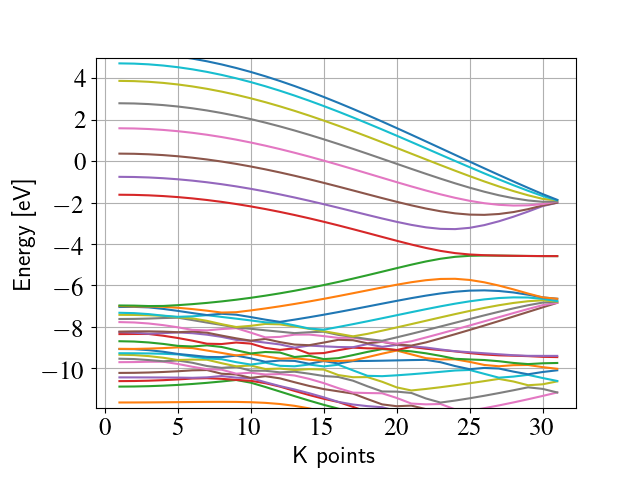
\includegraphics[width=0.700\linewidth]{zigzag-band.png}
\caption{Band structure of the zigzag nanoribbon}\label{electstruct:fig-zigzag-band}\end{figure}
\end{quote}

\section{Armchair nanoribbon with defects}
\label{electstruct:armchair-nanoribbon-with-defects}
We now investigate a hydrogen saturated armchair carbon nanoribbon,
examining both the perfect ribbon and two defective structures, each
with a vacancy at a different position in the ribbon. In order to keep
the tutorial short, we will not relax the vacancies, but will only
remove one atom from the perfect structure.


\subsection{Perfect armchair nanoribbon}
\label{electstruct:perfect-armchair-nanoribbon}

\subsubsection{Total energy and density of state}
\label{electstruct:total-energy-and-density-of-state}
{[}Working directory: \emph{elect/armchair/perfect\_density/}{]}

The steps to calculate the DOS of the perfect H-saturated armchair
nanoribbon are the same as for the zigzag case. First check the
geometry with the help of repeated supercells:

\begin{Verbatim}[commandchars=\\\{\}]
sh checkgeo.sh
\end{Verbatim}

You will see a repeated image of the perfect armchair nanoribbon unit
cell (Figure {\hyperref[electstruct:fig-armchair-perfect-geo]{\emph{\DUspan{}{Perfect armchair nanoribbon unit cell}}}} (\autopageref*{electstruct:fig-armchair-perfect-geo})).
\begin{quote}
\begin{figure}[htbp]
\centering
\capstart

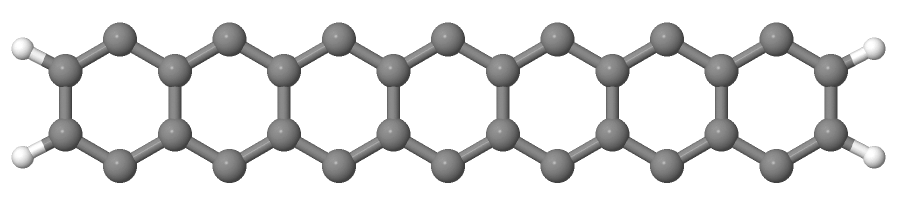
\includegraphics[width=0.700\linewidth]{armchair-perfect-geo.png}
\caption{Perfect armchair nanoribbon unit cell}\label{electstruct:fig-armchair-perfect-geo}\end{figure}
\end{quote}

The edge of the ribbon is visually different from the zigzag case. As
it turns out, this also has some physical consequences. Let's
calculate the electronic density and extract the density of states:

\begin{Verbatim}[commandchars=\\\{\}]
sh run.sh
\end{Verbatim}

If you look up the calculated Fermi-level and then visualize the DOS

\begin{Verbatim}[commandchars=\\\{\}]
sh showdos.sh
\end{Verbatim}

you can immediately see (Figure {\hyperref[electstruct:fig-armchair-perfect-dos]{\emph{\DUspan{}{DOS of the perfect armchair nanoribbon}}}} (\autopageref*{electstruct:fig-armchair-perfect-dos})) that
there are no states around the Fermi-energy (-4.4 eV), i.e. the
investigated armchair nanoribbon is non-metallic.
\begin{quote}
\begin{figure}[htbp]
\centering
\capstart
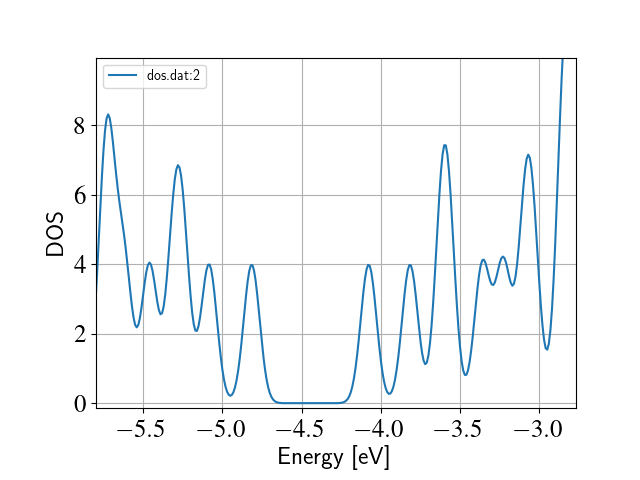
\includegraphics[width=0.650\linewidth]{armchair-perfect-dos.png}
\caption{DOS of the perfect armchair nanoribbon}\label{electstruct:fig-armchair-perfect-dos}\end{figure}
\end{quote}


\subsubsection{Band structure}
\label{electstruct:id2}
{[}Working directory: \emph{elect/armchair/perfect\_bands}{]}

Let's have a quick look at the band structure of the armchair
H-saturated ribbon. The steps are the same as for the zigzag case, so
just issue:

\begin{Verbatim}[commandchars=\\\{\}]
sh run.sh
sh showbands.sh
\end{Verbatim}

You should obtain a band structure like in Figure
{\hyperref[electstruct:fig-armchair-perfect-band]{\emph{\DUspan{}{The band structure of the perfect hydrogen passivated armchair
nanoribbon. The Fermi energy is at -4.4 eV.}}}} (\autopageref*{electstruct:fig-armchair-perfect-band}). You can read off the position of the
band edges, when you zoom into the energy region around the gap: The
valence band edge and the conduction band edge are in the Gamma point
at -4.7 and -4.2 eV, respectively. You can also easily extract this
information from the \emph{band.out} file, when you look where to
occupation goes from nearly 2.0 to nearly 0.0 in the first k-point
(the Gamma point).
\begin{quote}
\begin{figure}[htbp]
\centering
\capstart
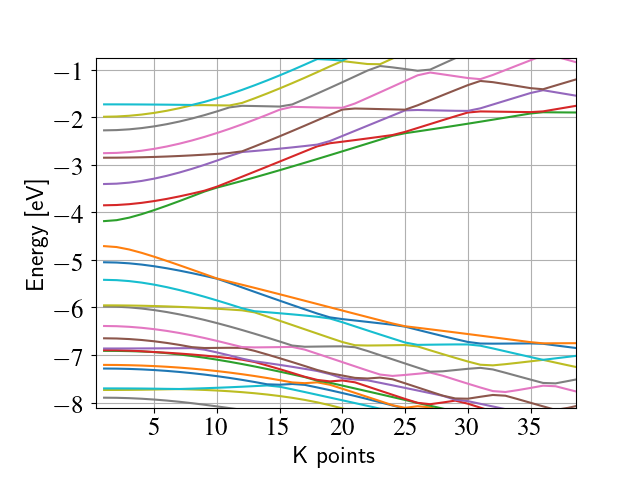
\includegraphics[width=0.650\linewidth]{armchair-perfect-band.png}
\caption{The band structure of the perfect hydrogen passivated armchair
nanoribbon. The Fermi energy is at -4.4 eV.}\label{electstruct:fig-armchair-perfect-band}\end{figure}
\end{quote}


\subsection{Armchair nanoribbon with vacancy}
\label{electstruct:armchair-nanoribbon-with-vacancy}

\subsubsection{Density and DOS}
\label{electstruct:density-and-dos}
{[}Working directory: \emph{elect/armchair/}{]}

As next, we should investigate two armchair nanoribbons with a vacancy
in each. The inputs can be found in the subdirectories
\emph{elect/armchair/vacancy1\_density} and
\emph{elect/armchair/vacancy2\_density} and you can visualize both with the
command

\begin{Verbatim}[commandchars=\\\{\}]
sh showgeom\PYGZus{}v12.sh
\end{Verbatim}

As you can see on Figures {\hyperref[electstruct:fig-armchair-v1-geo]{\emph{\DUspan{}{Armchair nanoribbon with vacancy (structure 1)}}}} (\autopageref*{electstruct:fig-armchair-v1-geo}) and
{\hyperref[electstruct:fig-armchair-v2-geo]{\emph{\DUspan{}{Armchair nanoribbon with vacancy (structure 2)}}}} (\autopageref*{electstruct:fig-armchair-v2-geo}), the vacancy is in the two cases on
different sublattices.
\begin{quote}
\begin{figure}[htbp]
\centering
\capstart

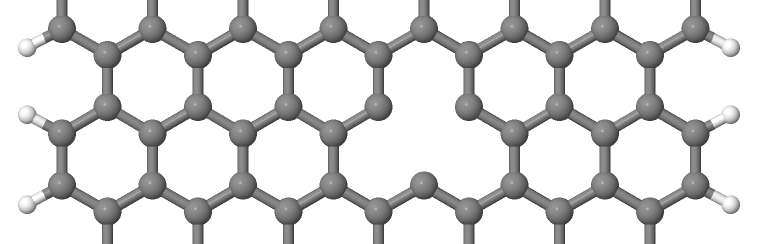
\includegraphics[width=0.700\linewidth]{armchair-v1-geo.png}
\caption{Armchair nanoribbon with vacancy (structure 1)}\label{electstruct:fig-armchair-v1-geo}\end{figure}
\begin{figure}[htbp]
\centering
\capstart

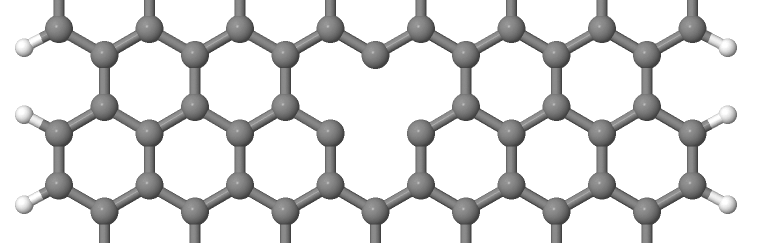
\includegraphics[width=0.700\linewidth]{armchair-v2-geo.png}
\caption{Armchair nanoribbon with vacancy (structure 2)}\label{electstruct:fig-armchair-v2-geo}\end{figure}
\end{quote}

The two vacancies (structures 1 and 2) are located on different
sublattices. Since the geometries are periodic along the z-direction,
the defects are also repeated. As we would like to calculate a single
vacancy, we have to make our unit cell for the defect calculation
large enough to avoid significant defect-defect interactions. In this
case, the defective cells contain twelve unit cells.

In order to calculate the electron density of both vacancies, issue:

\begin{Verbatim}[commandchars=\\\{\}]
sh run\PYGZus{}v12.sh
\end{Verbatim}

This will take slightly longer than the previous calculations, since
each system contains more than four hundred atoms.

We want to analyse the density of states of the two different
vacancies, together with that of the defect-free system. The commands
necessary to extract the DOS of all three configurations and show them
in one figure have been stored in the script
\code{showdos\_perf\_v12.sh}. Execute it

\begin{Verbatim}[commandchars=\\\{\}]
sh showdos\PYGZus{}perf\PYGZus{}v12.sh
\end{Verbatim}

to obtain a figure like Figure {\hyperref[electstruct:fig-armchair-dos]{\emph{\DUspan{}{The DOS of the perfect nanoribbon is indicated by solid blue
line, the DOS of the nanoribbons with vacancies with green and
red lines, respectively.}}}} (\autopageref*{electstruct:fig-armchair-dos}).
\begin{quote}
\begin{figure}[htbp]
\centering
\capstart
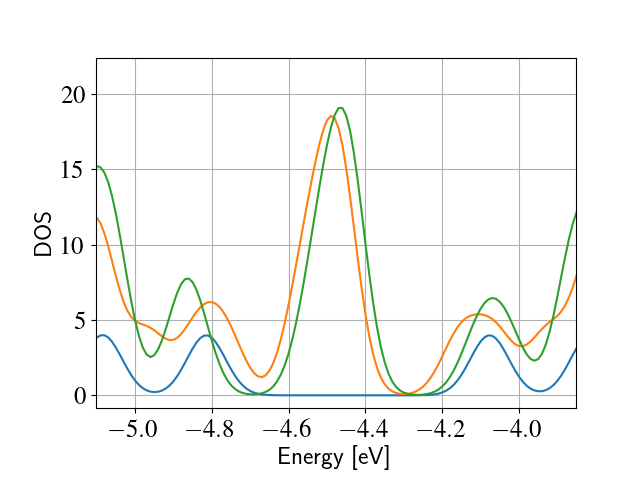
\includegraphics[width=0.700\linewidth]{armchair-dos.png}
\caption{The DOS of the perfect nanoribbon is indicated by solid blue
line, the DOS of the nanoribbons with vacancies with green and
red lines, respectively.}\label{electstruct:fig-armchair-dos}\end{figure}
\end{quote}

As you can see, in contrast to the zigzag nanoribbon, the perfect
armchair nanoribbon is insulating as it has no states around the
Fermi-energy (-4.45 eV).  The structures with vacancies, on the other
hand, introduce dangling (unsaturated) bonds, leading to unoccupied
states around the Fermi-energy. We can also see, that the defects
affect the band edges, which are shifted with respect to their
position in the perfect structure. It also seems that the valence band
edge is more affected than the conduction band edge, and in the case
of vacancy 2 (red line) the effect is significantly larger than for
vacancy 1 (green line).


\subsubsection{Vacancy formation energy}
\label{electstruct:vacancy-formation-energy}
You should also be able to calculate the formation energies of the two
vacancies. The formation energy \(E_{\text{form}}\) of the vacancy
in our case can be calculated as
$$
E_{\text{form}} = \left( E_{\text{vac}} + E_{\text{C}} \right)
- 12 \times E_{\text{perf}}
$$

where \(E_{\text{vac}}\) is the total energy of the nanoribbon
with the vacancy present, \(E_{\text{C}}\) is the energy of a
C-atom in its standard phase and \(E_{\text{perf}}\) is the energy
of the perfect nanoribbon. Since the defective nanoribbons contain 12
unit cell of the perfect one, the energy of the perfect ribbon unit
cell has to be multiplied by twelve. As a standard phase of carbon, we
will take perfect graphene for simplicity. The energy of the C-atom in
its standard phase is then obtained by dividing the total energy of
the perfect graphene primitive unit cell by two. (Look up this energy
from \emph{detailed.out} in the directory \emph{elect/graphene/density}.)  By
calculating the appropriate quantities you should obtain $\sim$8.5 eV for
the formation energy of both vacancies. This is quite a high value,
but you should recall that the vacancies have not been structurally
optimised, and their formation energies are therefore, significantly
higher than for the relaxed configurations.


\subsubsection{Defect levels}
\label{electstruct:defect-levels}
{[}Working directory: \emph{elect/armchair/vacancy2\_wf/}{]}

Finally we should identify the localised defect levels for vacancy 2
and plot the corresponding one-electron wavefunctions.

The vacancy was created by removing one C-atom, which had three first
neighbors. Therefore, three \emph{sp2} type dangling bonds remain in the
lattice, which will then form some linear combinations to produce
three defect levels, which may or may not be in the band gap. The DOS
you have plotted before, indicates there are indeed defect levels in
the gap, but due to the smearing it is hard to say how many they are.

We want to investigate the defect levels at the Gamma point, as this
is where the perfect nanoribbon has its band edges. We will therefore
do a quick Gamma-point only calculation for vacancy structure 2 using
the density we obtained before. We will set up the input to write out
also the eigenvectors (and some additional information) so that we can
plot the defect levels with \emph{waveplot} later. This needs the following
additional settings in \emph{dftb\_in.hsd}:

\begin{Verbatim}[commandchars=\\\{\}]
Options \PYGZob{}
  WriteEigenvectors = Yes
  WriteDetailedXML = Yes
  WriteDetailedOut = No
\PYGZcb{}
\end{Verbatim}

To just run the calculation

\begin{Verbatim}[commandchars=\\\{\}]
sh run.sh
\end{Verbatim}

and open the \emph{band.out} file. You will see, that you have three levels
(levels 742, 743 and 744 at energies of -4.51, -4.45 and -4.45 eV,
respectively) which are between the energies of the band edge states
of the perfect ribbon. We will visualize those three levels by using
the \emph{waveplot} tool.

Waveplot reads the eigenvectors produced by \dftbp and plots real space
wave functions and densities. The input file \emph{waveplot\_in.hsd} can be
used to control which levels and which region waveplot should
visualize, and on what kind of grid. In the current example, we will
project the real part of the wave functions for the levels 742, 743
and 744. In order to run Waveplot, enter:

\begin{Verbatim}[commandchars=\\\{\}]
waveplot \textbar{} tee output.waveplot
\end{Verbatim}

The calculation could again take a few minutes. At the end, you should
see three files with the \emph{.cube} prefix, containing the volumetric
information for the three selected one-electron wavefunctions.

We will use Jmol to visualize the various wave function
components. Unfortunately, the visualization of iso-surfaces in Jmol
needs some scripting. You can find the necessary commands in the files
\emph{show*.js}. You can either type in these commands in the Jmol console
(which should be opened via the menu \emph{File \textbar{} Console...}) or pass it
to Jmol using the \emph{-s} option at start-up. For the case latter you
will find prepared command to visualize the various orbitals in the
files

\begin{Verbatim}[commandchars=\\\{\}]
sh showdeflev1.sh && sh showdeflev2.sh && sh showdeflev3.sh
\end{Verbatim}

Looking at the defect levels, you can see that the defect level lowest
in energy (742) has a significant contribution on the atoms around the
defect, but also a non-negligible delocalized part smeared over almost
all atoms in the system. Apparently a localized defect level has
hybridized with the delocalized valence band edge state, resulting in
a mixture between localized and non-localized state. The other two
defect levels, on the other hand, have wavefunctions which are well
localized on the atoms around the vacancy site. Note that in
accordance with the overall symmetry of the system, the defect levels
are either symmetric or antisymmetric with respect to the mirror plane
in the middle of the ribbon.
\begin{quote}
\vskip -0.2cm
\begin{figure}[htbp]
\centering
\capstart
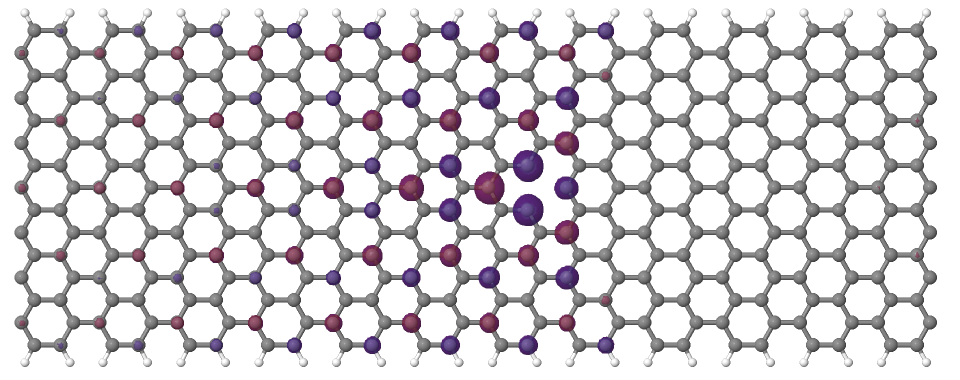
\includegraphics[width=0.650\linewidth]{armchair-v2-def1.png}
\caption{Wave function of the lowest defect level of the hydrogen
saturated armchair nanoribbon with a vacancy. Blue and red
surfaces show indicate isosurfaces at +0.02 and -0.02 atomic
units, respectively.}\label{electstruct:fig-armchair-v2-def1}
\end{figure}
\vskip -0.2cm
\begin{figure}[htbp]
\centering
\capstart
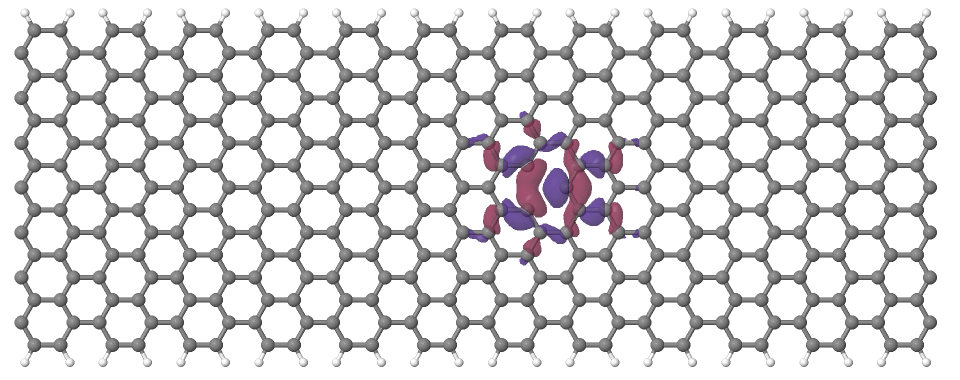
\includegraphics[width=0.650\linewidth]{armchair-v2-def2.png}
\caption{Wave function of the second lowest defect level of the hydrogen
saturated armchair nanoribbon with a vacancy.}\label{electstruct:fig-armchair-v2-def2}
\end{figure}
\vskip -0.2cm
\begin{figure}[htbp]
\centering
\capstart
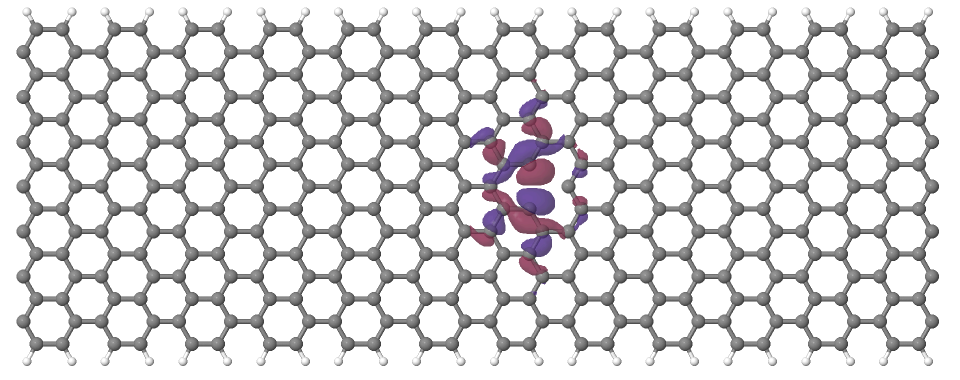
\includegraphics[width=0.650\linewidth]{armchair-v2-def3.png}
\caption{Wave function of the highest defect level of the hydrogen
saturated armchair nanoribbon with a vacancy.}\label{electstruct:fig-armchair-v2-def3}
\end{figure}
\end{quote}


\chapter{Electron transport calculations in armchair nanoribbons}
\label{transport::doc}\label{transport:electron-transport-calculations-in-armchair-nanoribbons}
In this sections of the tutorial we will learn how to set up self-consistent and non self-consistent simulations with open boundary conditions. We will then
calculate the density of states and the transmission coefficients and then
analyse the results in comparison with the previous periodic
calculations.

If you have not done so yet, please download the file
\emph{tutorial\_input.zip} and decompress it by issuing:

\begin{Verbatim}[commandchars=\\\{\}]
unzip tutorial\PYGZus{}input.zip
\end{Verbatim}

in some directory. Then enter the directory \emph{transport/}. All
directories given in this part of the tutorial are sub-directories of
the \emph{transport/} directory.


\section{Non-SCC Pristine armchair nanoribbon}
\label{transport:non-scc-pristine-armchair-nanoribbon}
{[}Working directory: \emph{transport/agr\_nonscc/ideal/}{]}


\subsection{Preparing the structure}
\label{transport:preparing-the-structure}
When we run a transport calculation with open boundary conditions, the
geometric structure specified in the input needs to obey some
rules. The system must consist of an extended device (or molecule)
region, and two or more semi-infinite bulk contacts. The bulk contacts
are described by providing two \emph{principal layers} for each contact.

A \emph{Principal Layer (PL)} is defined as a contiguous group of atoms
that have finite interaction only with atoms belonging to adjacent
PLs. In a sense, a PL is a generalisation of the idea of nearest
neighbour atoms to the idea of nearest neighbour blocks. The PL
partitioning in the electrodes is used by the code to retrieve a
description of the bulk system. PLs may be defined, as we will see, in
the extended device region to take advantage of the iterative Green
function solver algorithm.

Additional information about the definition of PLs, contacts and
extended device region can be found in the manual and in the on-line
recipes.

In the case of an ideal one-dimensional system, all the PLs are
identical. The system we start with is an infinite armchair graphene
nanoribbon (AGR), therefore the partitioning into device and contact
regions is somewhat arbitrary. We will therefore start from a
structure file containing a single PL (\emph{2cell\_7.gen}), which has been
previously relaxed. The PL can be converted to XYZ format by using the
\emph{gen2xyz} script and visualised with \emph{Jmol}:

\begin{Verbatim}[commandchars=\\\{\}]
gen2xyz 2cell\PYGZus{}7.gen
jmol 2cell\PYGZus{}7.xyz
\end{Verbatim}

The structure is shown in Figure {\hyperref[transport:fig-2cell-7]{\emph{\DUspan{}{Armchair nanoribbon principal layer (PL)}}}} (\autopageref*{transport:fig-2cell-7})
\begin{figure}[htbp]
\centering
\capstart

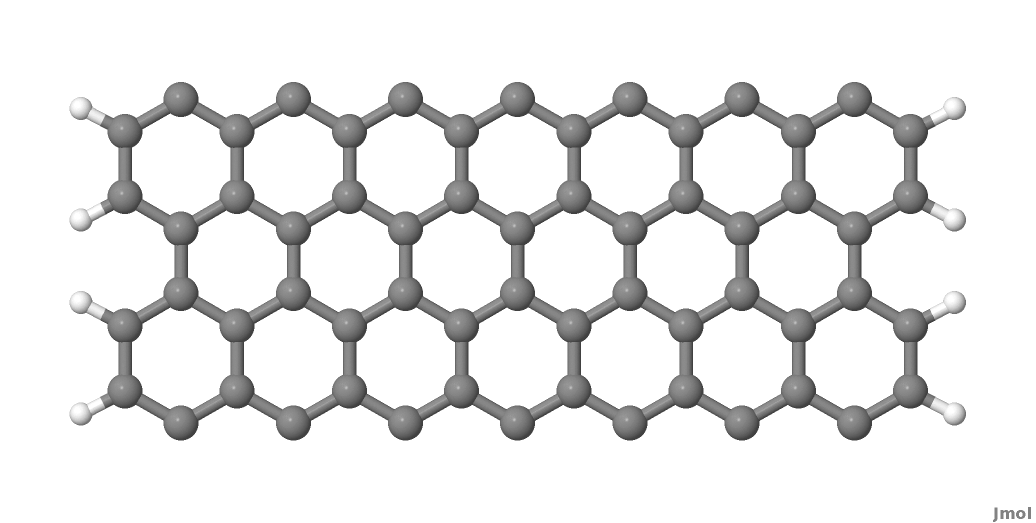
\includegraphics[width=0.600\linewidth]{2cell_7.png}
\caption{Armchair nanoribbon principal layer (PL)}\label{transport:fig-2cell-7}\end{figure}

As you may notice, we did not take a single unit cell length as a PL,
but rather two unit cells. This choice is dictated by the definition
of the PL itself, as we want to avoid non-zero interactions between
second-neighbour PLs. This is better explained by referring to Figure
{\hyperref[transport:fig-4cell-7]{\emph{\DUspan{}{Layer definition}}}} (\autopageref*{transport:fig-4cell-7}). The red carbon atoms represent the closest atoms
which would belong to non-nearest neighbour PLs, and these have a
separation of 0.568 nm, as shown in Figure {\hyperref[transport:fig-4cell-7]{\emph{\DUspan{}{Layer definition}}}} (\autopageref*{transport:fig-4cell-7}). The
carbon-carbon interaction is non zero up to a distance of 6 a.u.,
therefore the interaction between the two red atoms would be small,
but non zero. Hence this is too small a separation for a one unit cell
long section of nanoribbon to be used as the PL.
\begin{figure}[htbp]
\centering
\capstart

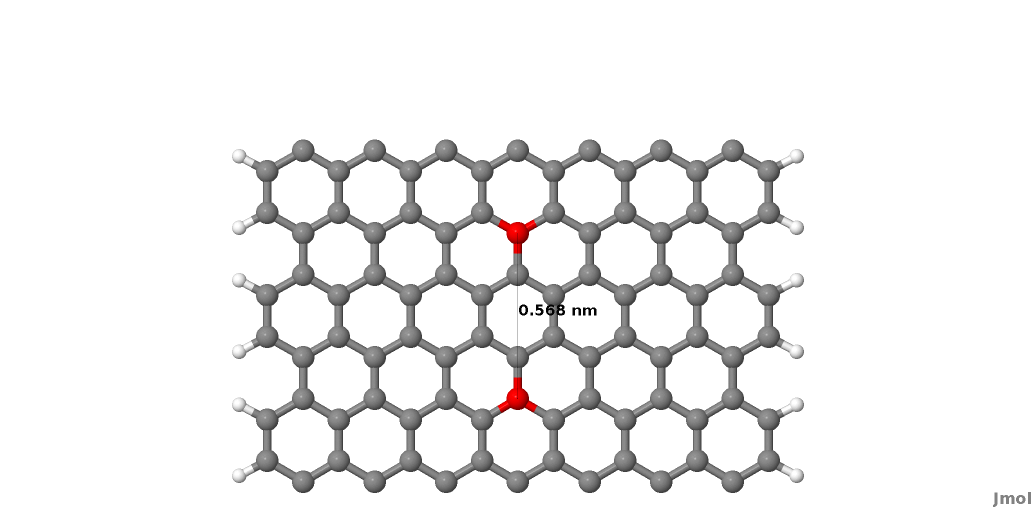
\includegraphics[width=0.800\linewidth]{4cell_7.png}
\caption{Layer definition}\label{transport:fig-4cell-7}\end{figure}

As currently there is no way to damp out small interactions, the PL
must contain two unit cells in this case, as shown in figure
{\hyperref[transport:fig-4cell-7]{\emph{\DUspan{}{Layer definition}}}} (\autopageref*{transport:fig-4cell-7}). It follows that the correct definition of a PL
depends both on the geometry of the system and the interaction cut-off
distance.

After having defined a proper PL, we then build a structure consisting
of a device region with 2 PLs and contacts at each end of this region,
each with 2 PLs.

\emph{Note}: For the pristine system, the equilibrium results should not
depend on the length of the device region, as the represented system
is an infinite ideal nanoribbon with discrete translational symmetry
along the ribbon.

The input atomic structure must be defined according to a specific
ordering: the device atoms come first, then each contact is specified,
starting with the PL closer to the device region. For an ideal system
defined by repetition of identical PLs, the tool \emph{buildwire}
(distributed with the code) can be used to build a 1D geometry with
the right ordering.

When you type:

\begin{Verbatim}[commandchars=\\\{\}]
buildwire 2cell\PYGZus{}7.gen
\end{Verbatim}

you will be asked to type the name of the file containing the input
supercell (\emph{2cell\_7.gen}) and the number of principal layers in the
device region (we will set this to be 2). \emph{buildwire} will always give
its output as a supercell structure, but in some cases we will need to
manually modify this structure file so that it corresponds to the
ordering explained in the previous paragraph.

The following output will be visualised:

\begin{Verbatim}[commandchars=\\\{\}]
Insert PL .gen file name:
2cell\PYGZus{}7.gen
Insert number of PLs in channel: 2
structure built
*iatc=
       137         272 0
       273         408 0
*PLs=
   1    69;
\end{Verbatim}

The indexes \textbf{iatc} and \textbf{PLs} define the atoms belonging to the
contacts, to the device region and to the PLs of the device region,
and will be useful when we will write the input files. You should take
a note of them (the iterative algorithm used in solving the Green
function requires these values). A file \emph{Ordered\_2cell\_7.gen} will
have been created, and defined as a supercell format GEN file (\code{S}),
which we will rename \emph{device\_7.gen} for the following:

\begin{Verbatim}[commandchars=\\\{\}]
mv Ordered\PYGZus{}2cell\PYGZus{}7.gen device\PYGZus{}7.gen
\end{Verbatim}

We can better
understand the ordering of the atomic indexes if we convert this
structure to XYZ, open it with jmol and then change the colours of
specific ranges of atoms by using the following syntax in the jmol
console (for example, we select here the first contact and split it
into two sub-ranges containing its first and second PLs):

\begin{Verbatim}[commandchars=\\\{\}]
\PYGZgt{} select atomno\PYGZgt{}136 \PYGZam{}\PYGZam{} atomno\PYGZlt{}205
\PYGZgt{} color yellow
\PYGZgt{} select atomno\PYGZgt{}204 \PYGZam{}\PYGZam{} atomno\PYGZlt{}273
\PYGZgt{} color red
\end{Verbatim}

In Figure {\hyperref[transport:fig-color-device-7]{\emph{\DUspan{}{The PLs of contact 1}}}} (\autopageref*{transport:fig-color-device-7}) a \emph{Jmol} export of the structure is shown.
\begin{figure}[htbp]
\centering
\capstart

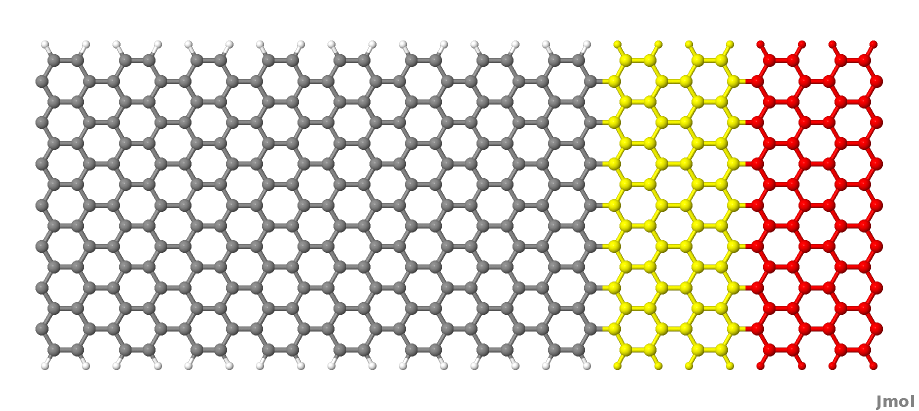
\includegraphics[width=0.800\linewidth]{color_device_7.png}
\caption{The PLs of contact 1}\label{transport:fig-color-device-7}\end{figure}

The yellow and red atoms represent the first and second PLs of the
first contact. When you build a structure yourself, it is always a
good idea to use a visualiser and verify that the atomic indices are
consistent with the transport setup definitions.

The last step is to change the supercell definition in the gen
structure file. From the point of view of an open boundary condition
calculation, Supercell (\code{S}) and Cluster (\code{C}) have a slightly
different meaning with respect to a canonical \emph{dftb} calculation. By
Supercell we mean any structure which is \emph{periodic in any direction
transverse to the transport direction}, while for cluster we mean any
structure \emph{not periodic in any direction transverse to transport}. It
follows that purely 1D systems, like nanowires and nanoribbons, should
be regarded as clusters (\code{C}). Therefore we edit the structure file
\emph{device\_7.gen}, changing in the first line the \code{S} (supercell) to be
\code{C} (cluster) and remove the last four lines, which would normally
only be defined for periodic systems.

This is the file we get after running \emph{buildwire}:

\begin{Verbatim}[commandchars=\\\{\}]
408  S
C    H
  1    1     37.831463060000    \PYGZhy{}20.000000000000      0.710000000000
  2    1     39.061219140000    \PYGZhy{}20.000000000000      1.420000000000
  3    1     39.061219140000    \PYGZhy{}20.000000000000      2.840000000000
  4    1     37.831463060000    \PYGZhy{}20.000000000000      3.550000000000
  5    1     35.371950920000    \PYGZhy{}20.000000000000      0.710000000000
  6    1     36.601706990000    \PYGZhy{}20.000000000000      1.420000000000
  7    1     36.601706990000    \PYGZhy{}20.000000000000      2.840000000000
  8    1     35.371950920000    \PYGZhy{}20.000000000000      3.550000000000
  ........
  65    2     20.880312110000    \PYGZhy{}20.000000000000    \PYGZhy{}11.870830122700
  66    2     20.880312110000    \PYGZhy{}20.000000000000     \PYGZhy{}9.429169877000
  67    2     40.025607920000    \PYGZhy{}20.000000000000    \PYGZhy{}11.870893735700
  68    2     40.025607920000    \PYGZhy{}20.000000000000     \PYGZhy{}9.429106264000
  0.000000000000000      0.000000000000000      0.000000000000000
  59.676097169999998        0.0000000000000000        0.0000000000000000
  0.0000000000000000       \PYGZhy{}40.000000000000000        0.0000000000000000
  0.0000000000000000        0.0000000000000000        51.119999999999997
\end{Verbatim}

Note that the numbering of atoms at the start of each line, as output
by \emph{buildwire} are sequential according to the numbering of the
initial structure, not its global position in the output file.

The corrected definition for the 1D ribbon with open boundary
conditions is then:

\begin{Verbatim}[commandchars=\\\{\}]
408  C
C    H
  1    1     37.831463060000    \PYGZhy{}20.000000000000      0.710000000000
  2    1     39.061219140000    \PYGZhy{}20.000000000000      1.420000000000
  3    1     39.061219140000    \PYGZhy{}20.000000000000      2.840000000000
  4    1     37.831463060000    \PYGZhy{}20.000000000000      3.550000000000
  5    1     35.371950920000    \PYGZhy{}20.000000000000      0.710000000000
  6    1     36.601706990000    \PYGZhy{}20.000000000000      1.420000000000
  7    1     36.601706990000    \PYGZhy{}20.000000000000      2.840000000000
  8    1     35.371950920000    \PYGZhy{}20.000000000000      3.550000000000
  ........
  65    2     20.880312110000    \PYGZhy{}20.000000000000    \PYGZhy{}11.870830122700
  66    2     20.880312110000    \PYGZhy{}20.000000000000     \PYGZhy{}9.429169877000
  67    2     40.025607920000    \PYGZhy{}20.000000000000    \PYGZhy{}11.870893735700
  68    2     40.025607920000    \PYGZhy{}20.000000000000     \PYGZhy{}9.429106264000
\end{Verbatim}

Now the file \emph{device\_7.gen} contains the correct structure, defined as
a cluster and with the proper atom ordering. Next, we set up the input
file for a tunnelling calculation.


\subsection{Transmission and density of states}
\label{transport:transmission-and-density-of-states}
In the \dftbp input format, settings related to a transport
calculation may be required to appear in separate sections of the
\emph{dftb\_in.hsd} file, depending on the functionality they invoke. In the
following we will set up the simplest open boundary condition
calculation: a calculation of transmission coefficients according to
the Landauer-Caroli formula, assuming a non-SCC DFTB hamiltonian. We
will analyse and comment the different sections contained in the file
\emph{dftb\_in.hsd}.

First, we have the specification of the geometry:

\begin{Verbatim}[commandchars=\\\{\}]
Geometry = GenFormat \PYGZob{}
\PYGZlt{}\PYGZlt{}\PYGZlt{} \PYGZsq{}device\PYGZus{}7.gen\PYGZsq{}
\PYGZcb{}
\end{Verbatim}

This follows the same rule as in a regular \dftbp calculation, except
for the fact that the structure should follow the specific
partitioning structure explained in the previous section.

Whenever an open boundary system is defined, we have to specify a
block named \emph{Transport} which contains information on the system
partitioning and additional information about the contacts to the
device:

\begin{Verbatim}[commandchars=\\\{\}]
Transport \PYGZob{}
  Device \PYGZob{}
    AtomRange = 1 136
    FirstLayerAtoms =  1 69
  \PYGZcb{}
  Contact \PYGZob{}
    Id = \PYGZdq{}source\PYGZdq{}
    AtomRange = 137 272
    FermiLevel [eV] = \PYGZhy{}4.7103
    potential [eV] = 0.0
  \PYGZcb{}
  Contact \PYGZob{}
    Id = \PYGZdq{}drain\PYGZdq{}
    AtomRange = 273 408
    FermiLevel [eV] = \PYGZhy{}4.7103
    potential [eV] = 0.0
  \PYGZcb{}
\PYGZcb{}
\end{Verbatim}

Here we have used the indexes printed by \emph{buildwire}. \emph{Device}
contains two fields: \emph{AtomRange} specifies which atoms belong to the
extended device region (1 to 136) and \emph{FirstLayerAtoms} specify the
starting index of the PLs in the device region. This field is
optional, but if not specified the iterative algorithm will not be
applied and the calculation will be slower, even though the result
will be still correct.  Then we have the definitions of the
contacts. In this example we define a two terminal system, but in
general N contacts are allowed. A contact is defined by an \emph{Id}
(mandatory), the range of atoms belonging to the contact specified in
\emph{AtomRange} (mandatory) and a \emph{FermiLevel} (mandatory). The potential
is set by default to 0.0, therefore need not be specified in this
example. Note that according to equilibrium Green function theory,
the Fermi level and the contact potential are not necessary to
calculate the transmission curve, but are required to calculate the
current via the Landauer formula, as they would determine the
occupation distribution in the contacts.

Then we have the \emph{Hamiltonian} block, which describes how the initial
Hamiltonian and the SCC component, if any, will be calculated:

\begin{Verbatim}[commandchars=\\\{\}]
Hamiltonian = DFTB \PYGZob{}
  SCC = No
  MaxAngularMomentum = \PYGZob{}
    C = \PYGZdq{}p\PYGZdq{}
    H = \PYGZdq{}s\PYGZdq{}
  \PYGZcb{}

  SlaterKosterFiles = Type2FileNames \PYGZob{}
    Prefix = \PYGZdq{}../../../sk/\PYGZdq{}  \PYGZsh{} To be substituted with the path to
                             \PYGZsh{} SK parameters on your local disk
    Separator = \PYGZdq{}\PYGZhy{}\PYGZdq{}
    Suffix = \PYGZdq{}.skf\PYGZdq{}
  \PYGZcb{}

  Eigensolver = TransportOnly\PYGZob{}\PYGZcb{}

\}
\end{Verbatim}

In this example we will calculate the transmission according to Caroli
(referred by some authors as Fisher Lee) formula in a non-SCC
approximation, i.e. the Hamiltonian is directly assembled from the
Slater-Koster files and used \emph{as is} to build the contact self
energies and the extended device Green function.  The definition of
an eigensolver is not meaningful in an open boundary setup, as the
system is instead solved by the Green function technique. Therefore
we just use a keyword \emph{TransportOnly} to indicate that we do not want
to solve an Eigenvalue problem. The other fields are filled up in the
same way as for a regular \dftbp calculation.

In general, in \dftbp an Eigensolver is regarded as a calculator
which can provide charge density in the SCC cycle, therefore we will
define a Green function based eigensolver later, but only for SCC
calculations.

Note that as C-H bonds are present in the system, charge transfer
should occur, hence the result will not be accurate at the non-SCC
level. It is not \emph{a-priori} trivial to predict whether this affects
qualitatively or quantitatively the transmission. We will therefore
later compare these results with an SCC calculation - at the moment we
will stay at the level of a non-SCC calculation, because it is faster
to execute and also allows us to use the simplest input file possible.

Finally, the implementation of the Landauer-Caroli formula is regarded
as a post-processing operation and specified by the block
\emph{TunnelingAndDos} inside \emph{Analysis}:

\begin{Verbatim}[commandchars=\\\{\}]
Analysis = \PYGZob{}
    TunnelingAndDos \PYGZob{}
      Verbosity = 101
      EnergyRange [eV] = \PYGZhy{}6.5  \PYGZhy{}3.0
      EnergyStep [eV] = 0.01
      Region = \PYGZob{}
        Atoms = 1:136
      \PYGZcb{}
    \PYGZcb{}
\PYGZcb{}
\end{Verbatim}

\emph{TunnelingAndDos} allows for the calculation of transmission
coefficient, Local Density of States (LDOS) and current. A
transmission is always calculated using the energy interval and energy
step specified here. The LDOS is only calculated when sub-blocks
\emph{Region} are defined. \emph{Region} can be used to select some specific
subsets of atoms or orbitals, according to the syntax explained in the
manual. In this example, we are specifying the whole extended device
region (atoms 1 to 136). Note that the energy range of interest is not
known a priori. Either you have a reference band structure
calculation, therefore you know where the first sub-bands are (this is
the correct way to do this), or you can run a quick calculation with a
large energy step and on the basis of the transmission curve then
refine the range of interest.

Now that the input file is complete, we have to complete one last
step. During a transport run, \dftbp will look for two directories
named \emph{GS} and \emph{contacts}. We have to create these directories in
advance:

\begin{Verbatim}[commandchars=\\\{\}]
mkdir GS
mkdir contacts
\end{Verbatim}

We can then start the calculation:

\begin{Verbatim}[commandchars=\\\{\}]
dftb+ dftb\PYGZus{}in.hsd \textbar{} tee output
\end{Verbatim}

We can take advantage of parallelisation over the energy points in the
calculation by running the code with \emph{mpirun}:

\begin{Verbatim}[commandchars=\\\{\}]
mpirun \PYGZhy{}n 4 dftb+ dftb\PYGZus{}in.hsd \textbar{} tee output
\end{Verbatim}

where \emph{4} should be substituted by the number of available nodes. Note
that Green function method is parallelised over energy points, therefore a number of
nodes larger than the energy grid will not improve performances and
secondly that the memory consumption is proportional to the number of
nodes used - this may be critical in shared memory systems with a
small amount of memory per node.

When the calculation has finished, the transmission and density of
states are saved to both the \emph{detailed.out} file and to two separate
\emph{tunneling.dat} and \emph{localDOS.dat} files. These additional files both
contain the energy points in the first column and the desired
quantities as additional columns.

We can plot the transmission by using the \emph{plotxy} script:

\begin{Verbatim}[commandchars=\\\{\}]
plotxy \PYGZhy{}\PYGZhy{}xlabel \PYGZsq{}Energy [eV]\PYGZsq{} \PYGZhy{}\PYGZhy{}ylabel \PYGZsq{}Transmission\PYGZsq{} \PYGZhy{}L tunneling.dat \&
\end{Verbatim}

The plot is shown in Figure {\hyperref[transport:fig-nonscc-tunn]{\emph{\DUspan{}{Non-SCC transmission through a pristine AGR}}}} (\autopageref*{transport:fig-nonscc-tunn}):
\begin{figure}[htbp]
\centering
\capstart
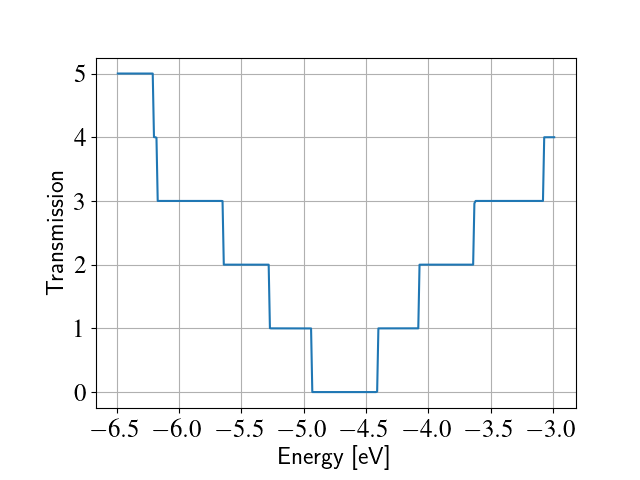
\includegraphics[width=0.700\linewidth]{nonscc-tunn.png}
\caption{Non-SCC transmission through a pristine AGR}\label{transport:fig-nonscc-tunn}\end{figure}

The ribbon is semiconducting, therefore we can see a zero transmission
at energies corresponding to the band gap. As the system is ideal,
outside of the band gap we can observe the characteristic conductance
steps where the value of the transmission is 1.0 for every band which
crosses a given energy. This is a normal signature of ideal 1D systems
with translational invariance.

Similarly, we can visualise the density of states by typing (the x and
y axis limits are chosen to focus on the first few sub-bands):

\begin{Verbatim}[commandchars=\\\{\}]
plotxy \PYGZhy{}\PYGZhy{}xlabel \PYGZsq{}Energy [eV]\PYGZsq{} \PYGZhy{}\PYGZhy{}ylabel \PYGZsq{}DOS [arbitrary units]\PYGZsq{} \PYGZhy{}L \PYGZbs{}
\PYGZhy{}\PYGZhy{}xlimits \PYGZhy{}6.5 \PYGZhy{}3 \PYGZhy{}\PYGZhy{}ylimit 0 1000 localDOS.dat \&
\end{Verbatim}

The result is shown in Figure {\hyperref[transport:fig-nonscc-dos]{\emph{\DUspan{}{Non-SCC density of states for a pristine AGR}}}} (\autopageref*{transport:fig-nonscc-dos}):
\begin{figure}[htbp]
\centering
\capstart
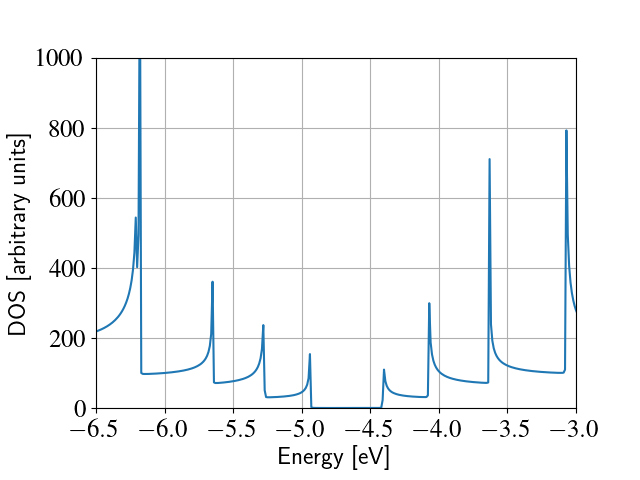
\includegraphics[width=0.700\linewidth]{nonscc-dos.png}
\caption{Non-SCC density of states for a pristine AGR}\label{transport:fig-nonscc-dos}\end{figure}

You can plot the transmission or the density of states on a
semi-logarithmic scale:

\begin{Verbatim}[commandchars=\\\{\}]
plotxy \PYGZhy{}\PYGZhy{}xlabel \PYGZsq{}Energy [eV]\PYGZsq{} \PYGZhy{}\PYGZhy{}ylabel \PYGZsq{}DOS [arbitrary units]\PYGZsq{} -L \PYGZbs{}
\PYGZhy{}\PYGZhy{}xlimits \PYGZhy{}6.5 \PYGZhy{}3 \PYGZhy{}\PYGZhy{}logscale y localDOS.dat \&
\end{Verbatim}

If you do so, you will obtain the plot shown in Figure
{\hyperref[transport:fig-nonscc-dos-semilogy]{\emph{\DUspan{}{Non-SCC density of states on logarithmic scale}}}} (\autopageref*{transport:fig-nonscc-dos-semilogy}).
\begin{figure}[htbp]
\centering
\capstart
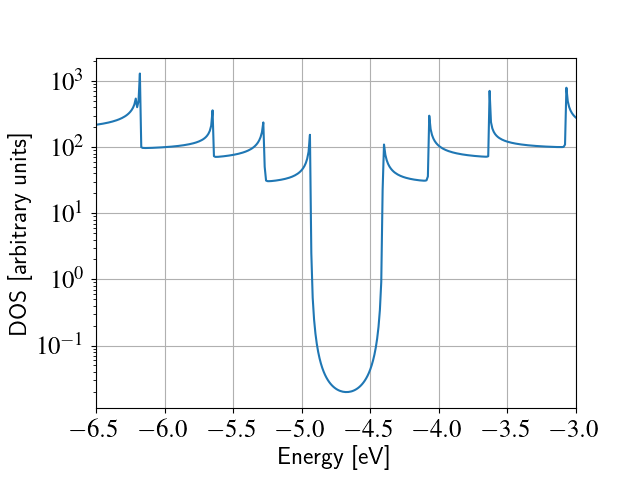
\includegraphics[width=0.700\linewidth]{nonscc-dos-semilog.png}
\caption{Non-SCC density of states on logarithmic scale}\label{transport:fig-nonscc-dos-semilogy}\end{figure}

The density of states in the band-gap is not zero, but decreases by
several orders of magnitude. This is a natural consequence of the
quasi-particle nature of the Green function formalism: every state
in the system has a finite broadening in energy.


\section{Non-SCC armchair nanoribbon with vacancy (A)}
\label{transport:non-scc-armchair-nanoribbon-with-vacancy-a}
{[}Working directory: \emph{transport/agr\_nonscc/vacancy1/}{]}


\subsection{Transmission and Density of States}
\label{transport:id1}
Now that we have a calculation of the reference pristine system, we
will introduce a scattering centre by producing a vacancy in the
system. In order to do so, we directly modify the structure file
\emph{device\_7.gen} and the input file \emph{dftb\_in.hsd}. We remove atom number
48 from the structure file. Note that \dftbp ignores the indexes in
the first column of the .gen file, therefore we do not need to adjust
them. We have, however, to remember to change the total number of
atoms in the first line from 408 to 407:

\begin{Verbatim}[commandchars=\\\{\}]
407  C
C    H
1    1     37.831463060000    \PYGZhy{}20.000000000000      0.710000000000
2    1     39.061219140000    \PYGZhy{}20.000000000000      1.420000000000
3    1     39.061219140000    \PYGZhy{}20.000000000000      2.840000000000
.....
46    1     32.912438770000    \PYGZhy{}20.000000000000      7.810000000000
47    1     30.452926620000    \PYGZhy{}20.000000000000      4.970000000000
49    1     31.682682700000    \PYGZhy{}20.000000000000      7.100000000000
50    1     30.452926620000    \PYGZhy{}20.000000000000      7.810000000000
...
\end{Verbatim}

The resulting structure should look like this:
\begin{figure}[htbp]
\centering
\capstart
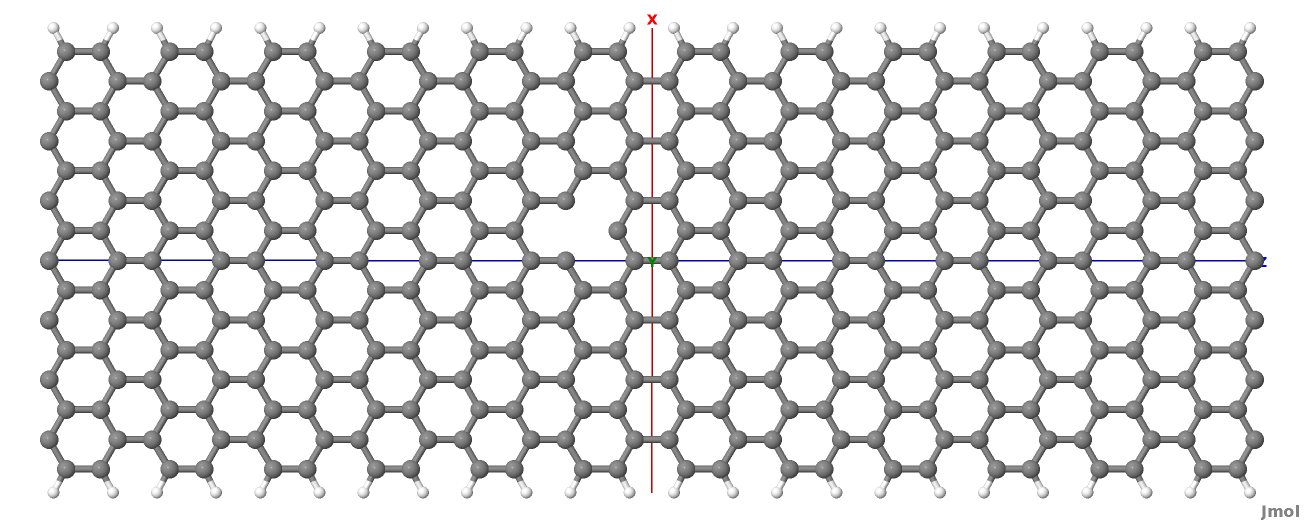
\includegraphics[width=0.800\linewidth]{device_7_vac.png}
\caption{Geometry with vacancy on sublattice A}\end{figure}

We then also adjust the dftb\_in.hsd file accordingly. As we have
removed an atom, all the indexes in the transport block need to be
adjusted properly. Note that we removed an atom in the first PL of the
extended device, therefore we also need to adjust the values of
FirstLayerAtoms. The \emph{Transport} block now reads:

\begin{Verbatim}[commandchars=\\\{\}]
Transport \PYGZob{}
    Device \PYGZob{}
      AtomRange = 1 135
      FirstLayerAtoms =  1 68
    \PYGZcb{}
    Contact \PYGZob{}
      Id = \PYGZdq{}source\PYGZdq{}
      AtomRange = 136 271
      FermiLevel [eV] = \PYGZhy{}4.7103
      potential [eV] = 0.0
    \PYGZcb{}
    Contact \PYGZob{}
      Id = \PYGZdq{}drain\PYGZdq{}
      AtomRange = 272 407
      FermiLevel [eV] = \PYGZhy{}4.7103
      potential [eV] = 0.0
    \PYGZcb{}
\PYGZcb{}
\end{Verbatim}

Compared to the pristine system, we have modified \emph{AtomRange} in all
the blocks and the values of \emph{FirstLayerAtoms}.

After running the
calculation, we can compare the transmission curve for this structure
with a single vacancy and the pristine ribbon by using plotxy:

\begin{Verbatim}[commandchars=\\\{\}]
plotxy \PYGZhy{}\PYGZhy{}xlabel \PYGZsq{}Energy [eV]\PYGZsq{} \PYGZhy{}\PYGZhy{}ylabel \PYGZsq{}Transmission\PYGZsq{} \PYGZhy{}L \PYGZhy{}\PYGZhy{}xlimits \PYGZhy{}6.5 \PYGZhy{}3 \PYGZbs{}
 ../ideal/tunneling.dat tunneling.dat \&
\end{Verbatim}
\begin{figure}[htbp]
\centering
\capstart
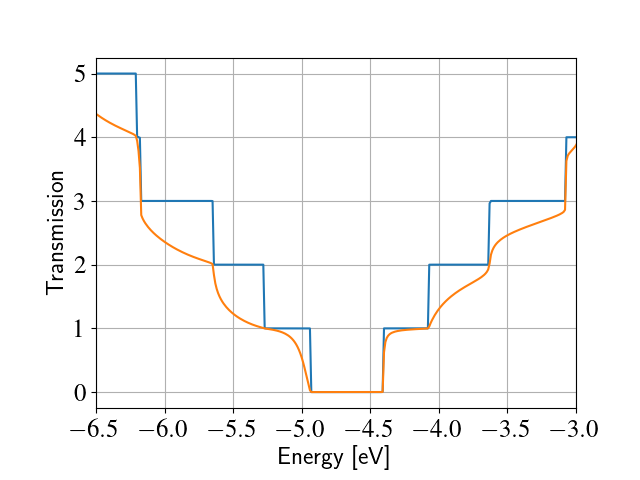
\includegraphics[width=0.700\linewidth]{nonscc-vac-tunn.png}
\caption{Non-SCC transmission in pristine (blue) and single vacancy (red) ribbons}\label{transport:fig-nonscc-vac-tunn}\end{figure}

Clearly, the presence of a vacancy introduces some finite scattering
which reduce the transmission with respect to the ideal ribbon.  In
particular, the effect is quite small in the first conductance band
while it is more visible in the first valence band and in higher
bands.  The reflection amplitude is increased near the band
edges. This is expected in 1D systems, as near the band edges the
density of states diverges (Van Hove singularities), hence the group
velocity is lower, and it is known from semi-classical transport
theory that the scattering probability is, when short range disorder
is present, inversely proportional to the group velocity. The absence
of resonant features in the transmission may point to the fact that
the vacancy does not induce additional states in the conduction or
valence bands. This can be verified by visualising the density of
states, as in Figure {\hyperref[transport:fig-nonscc-vac-dos]{\emph{\DUspan{}{Non-SCC DOS for single vacancy in sublattice A (linear scale)}}}} (\autopageref*{transport:fig-nonscc-vac-dos}).
\begin{figure}[htbp]
\centering
\capstart

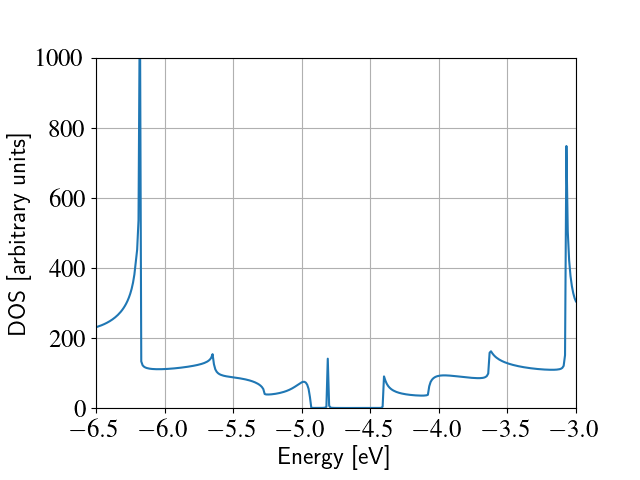
\includegraphics[width=0.700\linewidth]{nonscc-vac-dos.png}
\caption{Non-SCC DOS for single vacancy in sublattice A (linear scale)}\label{transport:fig-nonscc-vac-dos}\end{figure}

The same density of states can be visualised on logarithmic scale as
well, as in Figure {\hyperref[transport:fig-nonscc-vac-semilog-dos]{\emph{\DUspan{}{Non-SCC DOS for single vacancy on sublattice A (semilog scale)}}}} (\autopageref*{transport:fig-nonscc-vac-semilog-dos}).
\begin{figure}[htbp]
\centering
\capstart
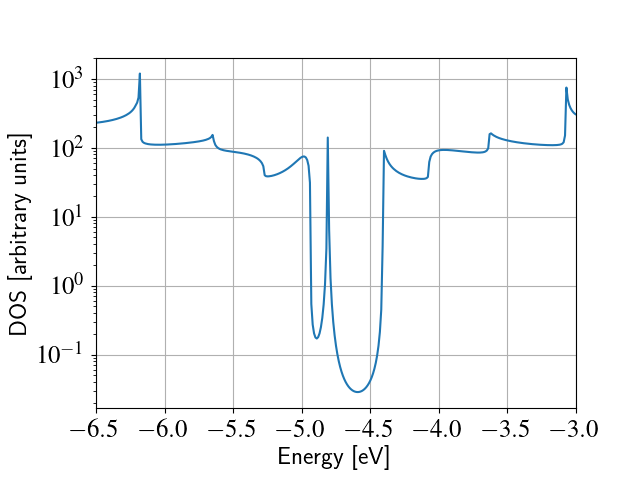
\includegraphics[width=0.700\linewidth]{nonscc-vac-semilog-dos.png}
\caption{Non-SCC DOS for single vacancy on sublattice A (semilog scale)}\label{transport:fig-nonscc-vac-semilog-dos}\end{figure}

The vacancy is adding some close energy levels in the gap, as verified
already from the \emph{DFTB} calculation in the first part of the
tutorial. The Van Hove singularities are partially suppressed as the
system no longer possesses translational symmetry along the transport
direction. Even in a simple non-SCC approximation, the qualitative
picture is consistent with the previous SCC periodic calculation. We
will now consider a vacancy sitting on the other sublattice (B) and
try to understand whether the relative position of the vacancy is
relevant or not by calculating once more the non-SCC transmission and
density of states

\newpage
\section{Non-SCC armchair nanoribbon with vacancy (B)}
\label{transport:non-scc-armchair-nanoribbon-with-vacancy-b}
{[}Working directory: \emph{transport/agr\_nonscc/vacancy2/}{]}


\subsection{Transmission and Density of States}
\label{transport:id2}
We will now consider a vacancy sitting on the other sublattice (B),
i.e. we can take the structure file we used for the ideal ribbon and
delete the atom number 47. The structure file is:

\begin{Verbatim}[commandchars=\\\{\}]
407  C
C    H
1    1     37.831463060000    \PYGZhy{}20.000000000000      0.710000000000
2    1     39.061219140000    \PYGZhy{}20.000000000000      1.420000000000
3    1     39.061219140000    \PYGZhy{}20.000000000000      2.840000000000
.....
46    1     32.912438770000    \PYGZhy{}20.000000000000      7.810000000000
48    1     31.682682700000    \PYGZhy{}20.000000000000      5.680000000000
49    1     31.682682700000    \PYGZhy{}20.000000000000      7.100000000000
50    1     30.452926620000    \PYGZhy{}20.000000000000      7.810000000000
.....
\end{Verbatim}

The \emph{jmol} rendering of the geometry:
\begin{figure}[htbp]
\centering
\capstart
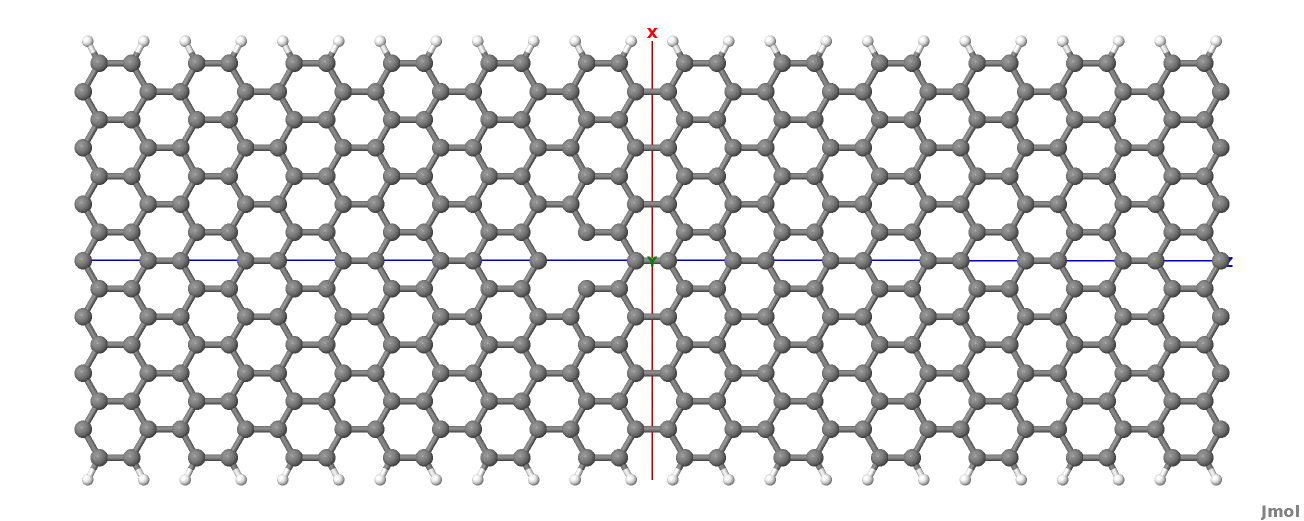
\includegraphics[width=0.800\linewidth]{device_7_vac2.png}
\caption{Geometry with vacancy on sublattice B}\end{figure}

Also in this case we remove an atom from the first PL of the extended
device region, therefore the rest of the \emph{dftb\_in.hsd} input file is
identical to the one we used for the vacancy on sublattice A. We can
therefore just copy it and run the \emph{dftb} calculation. The
transmission is shown in Figure {\hyperref[transport:fig-nonscc-vac2-tunn]{\emph{\DUspan{}{Non-SCC transmission for vacancy B (green), pristine (blue) and vacancy A (red)}}}} (\autopageref*{transport:fig-nonscc-vac2-tunn})
(Transmission for vacancy on sublattice B in blue, transmission for
vacancy on sublattice A in green and pristine system in green):
\begin{figure}[t]
\centering
\capstart
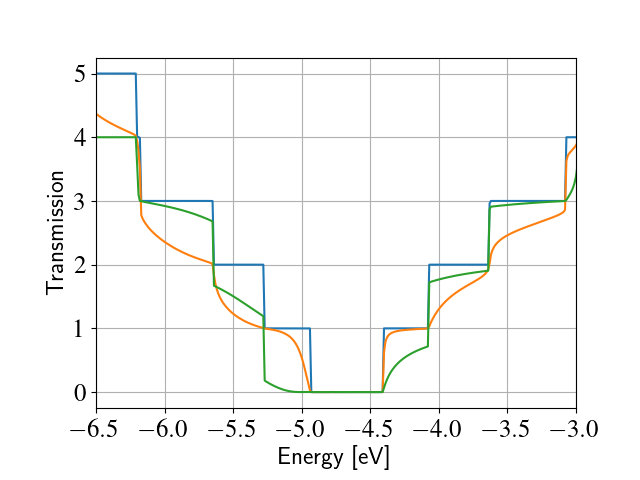
\includegraphics[width=0.700\linewidth]{nonscc-vac2-tunn.png}
\caption{Non-SCC transmission for vacancy B (green), pristine (blue) and
vacancy A (red)}\label{transport:fig-nonscc-vac2-tunn}\end{figure}

We can see a very strong suppression of transmission in the first
sub-bands, especially in the first valence band. Again, the absence of
resonances may be due by gap states. In fact, we can verify it by
plotting the density of states, as shown in Figure
{\hyperref[transport:fig-nonscc-vac2-dos]{\emph{\DUspan{}{Non-SCC DOS for vacancy in sublattice B (semilog scale)}}}} (\autopageref*{transport:fig-nonscc-vac2-dos}).

We can clearly see that the vacancy induces some nearly degenerate gap
states, and that the density of states at higher energies is largely
unaffected. It is known that the relative position of a scattering
centre in a graphene nanoribbon with respect to different sub-lattices
strongly affects its scattering properties, as is shown in these
non-SCC calculation. Qualitatively, the picture is also consistent
with periodic calculations, with the difference that we obtain
directly information on the effect on transport properties via
transmission function. This also ensures that we do not have to worry
about choosing the right supercell or k-point sampling as the open
boundary conditions represent exactly the infinite system with a
single scattering centre. As already pointed out earlier, there is no
warranty that a non-SCC calculation give the proper result in a system
if relevant charge transfer is occurring, and in general it will
not. Therefore in the next section we will repeat the same calculation
by solving the SCC problem.

\begin{figure}[h]
\centering
\capstart
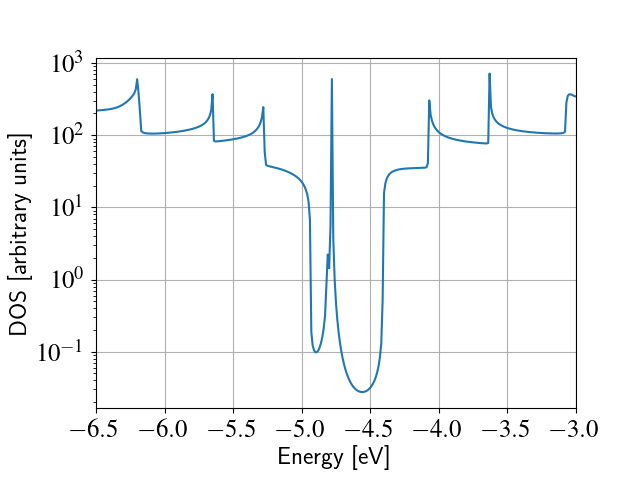
\includegraphics[width=0.700\linewidth]{nonscc-vac2-dos.png}
\caption{Non-SCC DOS for single vacancy on sublattice B (semilog scale)}\label{transport:fig-nonscc-vac2-dos}\end{figure}


\section{SCC Pristine armchair nanoribbon}
\label{transport:scc-pristine-armchair-nanoribbon}
A \emph{DFTB} Hamiltonian is in general given by two terms:
\begin{gather}
\begin{split}H^{SCC}=H^{0}+H^{shift}\end{split}\notag
\end{gather}
Where the component \(H^{shift}\) is the self-consistent (SCC)
correction. The SCC correction is in general needed whenever there is
a finite charge transfer between atoms, i.e. whenever there are bonds
between atoms with different chemical species or with different
coordination numbers. In our case, we can expect a finite charge
transfer between the C and H atoms at the edges, and an SCC component
may be relevant. While in the previous sections, we have only
considered the non-SCC component \(H^{0}\), in the next sections
we will compute the same calculation by including the correction given
by the shifts \(H^{shifts}\).

Note that the equilibrium SCC problem can be tackled in two ways: we
could apply the Landauer-Caroli to an SCC Hamiltonian taken, for
example, from a periodic calculation (i.e. uploading the SCC
component), or we can solve the problem as a full NEGF setup with 0
bias. The code flow is currently such that this second procedure has
to be used (however, the first technique will be available in future
release). Therefore we will need to learn to set the input related to
two other components of the NEGF machinery: the real space Poisson
solver and the Green function density matrix.

In this way we will introduce a first complete input file. It is
important, from a didactic point of view, to be clear that as long as
the applied bias is zero and we are interested in equilibrium
properties, the two approaches are equivalent and the results are only
valid in the limit of linear response.


\subsection{Contact calculation}
\label{transport:contact-calculation}
{[}Working directory: \emph{transport/agr\_scc/contacts/}{]}

In order to run an SCC transport calculation, the code needs some
additional knowledge about the contact PLs. In particular, the SCC
shifts and Mulliken charges have to be saved somewhere to enable
consistency between the calculation of the self-energy and the
calculation of the Poisson potential. To this end, we have to
introduce an additional step in the procedure: the contact
calculation.

The contact calculation is simply a \emph{DFTB} periodic calculation for
the contact PL. As such, not all the field defined in the transport
are meaningful and the input file will of course look different. The
\emph{Geometry} block is identical:

\begin{Verbatim}[commandchars=\\\{\}]
Geometry = GenFormat \PYGZob{}
\PYGZlt{}\PYGZlt{}\PYGZlt{} \PYGZsq{}device\PYGZus{}7.gen\PYGZsq{}
\PYGZcb{}
\end{Verbatim}

While the \emph{Transport} block needs to be modified as follows:

\begin{Verbatim}[commandchars=\\\{\}]
Transport \PYGZob{}
    Device \PYGZob{}
      AtomRange = 1 136
    \PYGZcb{}
    Contact \PYGZob{}
      Id = \PYGZdq{}source\PYGZdq{}
      AtomRange = 137 272
    \PYGZcb{}
    Contact \PYGZob{}
      Id = \PYGZdq{}drain\PYGZdq{}
      AtomRange = 273 408
    \PYGZcb{}
  Task = ContactHamiltonian\PYGZob{}
     ContactId = \PYGZdq{}source\PYGZdq{}
  \PYGZcb{}
\PYGZcb{}
\end{Verbatim}

We first notice the addition of an option \emph{Task
=ContactHamiltonian\{...\}}, which was previously absent. This block
specifies that we intend to calculate the bulk contact SCC properties,
and the field \emph{ContactId} specifies which contact we want to
calculate. The field \emph{FirstLayerAtoms} in the \emph{Device} block is absent
(it does not make sense in a contact calculation) and so are the
fields \emph{FermiLevel} and \emph{Potential} in the two \emph{Contact} sections, as
they are not meaningful during this step. In general, the philosophy
of a \emph{DFTB} input file is that if input fields that would be useless
or contradictory are present, the code will halt with an error
message.

The Hamiltonian block shows some differences, too:

\begin{Verbatim}[commandchars=\\\{\}]
Hamiltonian = DFTB \PYGZob{}
  SCC = Yes
  SCCTolerance = 1e\PYGZhy{}6
  EwaldParameter = 0.1
  MaxAngularMomentum = \PYGZob{}
    C =\PYGZdq{}p\PYGZdq{}
    H = \PYGZdq{}s\PYGZdq{}
  \PYGZcb{}

  SlaterKosterFiles = Type2FileNames \PYGZob{}
  Prefix = \PYGZdq{}../../../sk/\PYGZdq{}
  Separator = \PYGZdq{}\PYGZhy{}\PYGZdq{}
  Suffix = \PYGZdq{}.skf\PYGZdq{}
\PYGZcb{}

  KpointsAndWeights = SupercellFolding\PYGZob{}
   25 0 0
    0 1 0
    0 0 1
    0.0 0.0 0.0
  \PYGZcb{}
\PYGZcb{}
\end{Verbatim}

The flags \emph{SCC=Yes} and \emph{SCCTolerance=1e-6} enable the SCC
calculation.  A small tolerance in the contact calculation, and in
general in transport calculation, helps to avoid artificial mismatches
at device/contact boundaries.  The parameter \emph{EwaldParameter} needs to
sometimes be set when using parallel calculations to reduce the size
of the neighbour list. Typically, the code may complain about a too
small parameter: in that case, setting a value of 0.1 is considered to
be good practice. The other parameters are the usual ones, except for
the \emph{KPointsAndWeight}, which deserves special attention.

The bulk contact is of course a periodic structure, hence we need to
specify a proper k-point sampling, as we would do in a regular
periodic \emph{DFTB} calculation. However, you should be careful about the
way the lattice vector is internally defined. In the input system is a
cluster (C), i.e. \emph{it has no periodicity in direction transverse to
the transport directions}, the lattice vector of the contact is
internally reconstructed and assigned to be the first lattice vector,
\emph{regardless the spatial orientation of the structure}. This means that
the \emph{KPointsAndWeights} for a cluster system are always defined as
above: a finite number of k-points along the first reciprocal vector
(according to a 1D Monkhorst-Pack scheme) and a Gamma point sampling
along the other two directions. The reason for this choice is that we
do not want to assign a specific direction to the structures, i.e. at
this level we do not assume in any way that the structure must be
oriented along x,y or z direction.

Note also that as the contact information is used in the transport
calculation, it is a good idea to use a dense k point sampling and a
low SCC tolerance, in order to get a very well converged solution. The
contact calculation will be usually much faster than the transport
calculation, so this does not usually present a problem.

On the other hand, this rule regarding k-points does not apply to
periodic transport calculations, as the periodicity along the
transverse directions must also be preserved (refer to the following
section for a periodic system example). We can run the calculation by
typing:

\begin{Verbatim}[commandchars=\\\{\}]
dftb+ dftb\PYGZus{}in.hsd \textbar{}tee output
\end{Verbatim}

After running the calculation, we notice that a file
\emph{shiftcont\_source.dat} is generated. This file contains the
information useful for the transport calculation (shifts and charges
of a bulk contact). It is suggested you also keep a copy of the
\emph{detailed.out} for later reference. We can obtain the value of the
Fermi energy, which we will later need, from \emph{detailed.out} as -4.7103
eV.

We can now run the same calculation for the drain contact by just
modifying the \emph{Task} block:

\begin{Verbatim}[commandchars=\\\{\}]
Task = ContactHamiltonian\PYGZob{}
     ContactId = \PYGZdq{}drain\PYGZdq{}
  \PYGZcb{}
\end{Verbatim}

The contact are identical, therefore we expect the same results, also
with the same Fermi energy. We now have a file \emph{shiftcont\_drain.out},
which is equivalent to \emph{shiftcont\_drain.dat} apart from small
numerical error. In fact, we could have simply copied the previous
contact results into this file.

Now that the contact calculation is available, we can set up the
transport calculation.


\subsection{Transmission and Density of States}
\label{transport:id3}
{[}Working directory: \emph{transport/agr\_scc/ideal/}{]}

In order to calculate the transmission for the SCC system, we have to
copy the files \emph{shiftcont\_drain.dat} and \emph{shiftcont\_source.dat} into
the current directory:

\begin{Verbatim}[commandchars=\\\{\}]
cp ../contacts/shiftcont* .
\end{Verbatim}

Then, we have to specify some additional blocks with respect to a
non-SCC calculation. We first look at the \emph{Transport} block.:

\begin{Verbatim}[commandchars=\\\{\}]
Transport \PYGZob{}
  Device \PYGZob{}
    AtomRange = 1 136
    FirstLayerAtoms =  1 69
  \PYGZcb{}
  Contact \PYGZob{}
    Id = \PYGZdq{}source\PYGZdq{}
    AtomRange = 137 272
    FermiLevel [eV] = \PYGZhy{}4.45
    potential [eV] = 0.0
  \PYGZcb{}
  Contact \PYGZob{}
    Id = \PYGZdq{}drain\PYGZdq{}
    AtomRange = 273 408
    FermiLevel [eV] = \PYGZhy{}4.45
    potential [eV] = 0.0
  \PYGZcb{}
  Task = UploadContacts \PYGZob{}
  \PYGZcb{}
\PYGZcb{}
\end{Verbatim}

The atom indices are of course the same, as the geometry of the system
is not changed. This time though, we explicitly specified a \emph{Task}
block named \emph{UploadContacts}, which declares that we are now running a
full transport calculation. \emph{Task=UploadContacts\{\}} is the default and
does not take any additional parameters, therefore you can safely omit
it.

Now that we are solving the full SCC scheme, we will allow for charge
transfer between the open leads and the extended device region,
therefore it is important to set a well-defined Fermi energy. While
this does not make any difference in a non-SCC transmission
calculation, it is crucial for the SCC calculation. A wrong or
unphysical Fermi energy will lead to unphysical charge accumulation or
depletion in the system.

To this end, you will have to pay some attention to the definition of
the Fermi energy. As we are calculating a semiconductor system, the
Fermi level should be in the energy gap. By calculating a band
structure or by inspection of the eigenvalues in the file
\emph{detailed.out} you can verify that the value -4.7103 is on the edge of
the conduction band. This can be explained as numerically the Fermi
level is defined by filling the single particle states till the
reference density is reached, therefore its position inside the gap of
a semiconductor is arbitrary. Therefore, while in metallic system we
may ensure consistency and use a well calculated Fermi level at some
specific temperature during all our transport calculation, in the case
of a semiconductor system we can manually set the Fermi level in the
middle of the energy gap (for this system, roughly at -4.45 eV) and
freely vary the temperature as long as the gap is larger than several
times the value of kT.

We will see in the following that there are some ways to verify that
the Fermi level is defined consistently, as this is often source of
confusion. Note also that, differently from other codes, \emph{dftb+} allows
for different Fermi levels in different contacts, which can be useful
when heterogeneous contacts are defined (for example, in a PN
junction). In that case a built-in potential is internally added to
ensure no current flow at equilibrium.

In the \emph{Hamiltonian} block now an SCC calculation has to be
specified:

\begin{Verbatim}[commandchars=\\\{\}]
Hamiltonian = DFTB \PYGZob{}
  SCC = Yes
  SCCTolerance = 1e\PYGZhy{}6
  ReadInitialCharges = No
  MaxAngularMomentum = \PYGZob{}
    C = \PYGZdq{}p\PYGZdq{}
    H = \PYGZdq{}s\PYGZdq{}
  \PYGZcb{}

  SlaterKosterFiles = Type2FileNames \PYGZob{}
  Prefix = \PYGZdq{}../../../sk/\PYGZdq{}
  Separator = \PYGZdq{}\PYGZhy{}\PYGZdq{}
  Suffix = \PYGZdq{}.skf\PYGZdq{}
  \PYGZcb{}
  ....
\end{Verbatim}

\emph{MaxAngularMomentum} and \emph{SlaterKosterFiles} are not modified. But
differently from the non-SCC calculation, we now need to specify a way
to solve the Hartree potential and the charge density
self-consistently. In a NEGF calculation, we use a real-space Poisson
solver to calculate the potential, and a Green function integration
method to calculate the density matrix:

\begin{Verbatim}[commandchars=\\\{\}]
...
Electrostatics = Poisson \PYGZob{}
  Poissonbox [Angstrom] = 40.0 30.0 30.0
  MinimalGrid [Angstrom] = 0.5 0.5 0.5
  SavePotential = Yes
\PYGZcb{}

Eigensolver = GreensFunction \PYGZob{}
  \PYGZcb{}

Mixer = Broyden \PYGZob{}
   MixingParameter = 0.02
 \PYGZcb{}
\PYGZcb{}
...
\end{Verbatim}

The Poisson section contains the definition of the real space grid
parameters. Note that differently from a normal \emph{dftb+} calculation,
simulating regions of vacuum is not for free, as the simulation domain
must be spanned by the real space grid. The grid is always oriented
along the orthogonal cartesian coordinate system. \emph{Poissonbox}
specifies the lateral length of the grid. The length along the
transport direction is ignored as it is automatically determined by
the code (in this case, z=30.0). The length along the transverse
direction are relevant and \emph{should be carefully set}. In order not to
force unphysical boundary conditions, you may extend the grid at least
1 nm away. If a strong charge transfer is present, you may go for a
larger grid according to your available computational resources. A
poorly defined grid can lead to no convergence at all, to a very
strange (and slow) convergence path or to unphysical
results. \emph{MinimalGrid} specifies the minimum step size for the
multigrid algorithm. Values between 0.2 and 0.5 are usually good,
where a lower value stands for higher precision. \emph{SavePotential = Yes}
will return a file containing the potential and charge density
profile, for later reference. These files can be quite large,
therefore the default is \emph{No}.

The Eigensolver is now specified as \emph{GreensFunction}. With this
definition, we instruct the code not to solve an eigenvalue problem
but rather to calculate the density matrix by integration of the
Keldysh Green function. This block provides the SCC charge density
with or without applied bias. The options define the integration
path. Usually the default options are good enough in most cases and
advanced users may refer to the manual and references therein.

The \emph{Mixer} options is present in \emph{dftb} calculations as
well. Convergence is known to be critical in NEGF schemes. In that
case, a lower \emph{MixingParameter} value will help to avoid strong
oscillation in the SCC iterations.

The last block is \emph{Analysis}:

\begin{Verbatim}[commandchars=\\\{\}]
...
Analysis = \PYGZob{}
  TunnelingAndDos \PYGZob{}
    Verbosity = 101
    EnergyRange [eV] = \PYGZhy{}6.0  \PYGZhy{}3.0
    EnergyStep [eV] = 0.01
  \PYGZcb{}
\PYGZcb{}
\end{Verbatim}

This block is identical to the non-scc calculation as the same task is
performed: calculation of transmission, current and DOS by using the
Landauer-Caroli formula. The transmission will be of course be
different due to the fact that the ground state charge density is now
solution of the SCC Hamiltonian and we have slightly changed the
energy range as the SCC component introduce a shift of the
band-structure (try to compare the SCC and non-SCC transmission results
when you are done). We can now run the calculation (after defining the
directories GS and contacts):

\begin{Verbatim}[commandchars=\\\{\}]
mkdir GS
mkdir contacts
dftb+ dftb\PYGZus{}in.hsd \textbar{}tee output
\end{Verbatim}

or:

\begin{Verbatim}[commandchars=\\\{\}]
mpirun \PYGZhy{}n 4 dftb+ dftb\PYGZus{}in.hsd \textbar{}tee output
\end{Verbatim}

Where \emph{-n 4} should be adapted to the number of available nodes. As
transport calculations in \emph{dftb+} are parallelised on energy points, a
quantity larger than 40 (the default number of integration points at
equilibrium) will not speed up the calculation of the density matrix.

An inspection of the file \emph{detailed.out} reveals that we have
additional information with respect to the non-SCC calculation,
including a list of atomic charges and orbital population, as now the
SCC density matrix has been calculated. The transmission is also saved
as separate file, and is shown in Figure {\hyperref[transport:fig-scc-tunn]{\emph{\DUspan{}{SCC (red) and Non-SCC (blue) transmission through pristine AGR}}}} (\autopageref*{transport:fig-scc-tunn}).
\begin{figure}[htbp]
\centering
\capstart
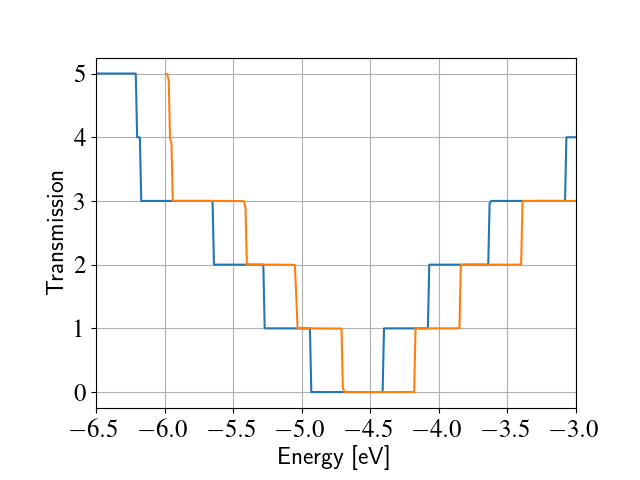
\includegraphics[width=0.800\linewidth]{scc-tunn.png}
\caption{SCC (red) and Non-SCC (blue) transmission through pristine AGR}\label{transport:fig-scc-tunn}\end{figure}

As you'd expect, it still step-like as in the non-SCC
calculation. This is correct, as we're calculating an ideal 1D
system. The bandwidth (i.e., the steps width) may differ due to SCC
contribution and the overall transmission is shifted. Note that while
the non-SCC calculation is very robust, meaning that you will always
get step-like transmission for a 1D system, in the SCC calculation a
poor definition of the boundary conditions, of the bulk contact
properties or of the additional \emph{GreensFunction} and \emph{Poisson} blocks
may induce numerical artifacts and scattering barriers which should
not be there. As a result, the transmission will not appear step-like
but rather visibly smoothed out.

You can also verify the quality of the calculation by inspection of
the potential and charge density profiles. In a pristine periodic
system we would expect a periodic potential, without discontinuities
at the boundary between extended device and electrodes. The
information needed to construct the real space potential and charge
density are contained in 5 files: \emph{box3d.dat}, \emph{Xvector.dat},
\emph{Yvector,dat}, \emph{Zvector.dat}, \emph{potential.dat} and
\emph{charge\_density.dat}. The first 4 files contain the grid information,
and the last two ones the list of potential and charge density values
(following a row major order). Those information can be converted to
any useful with some simple scripting, we provide an utility called
\emph{makecube} which can be used to convert them to Gaussian \emph{cube} format
or a more flexible \emph{vtk} format. There's plenty of software to
visualise \emph{vtk} or \emph{cube} files, but unluckily at present current
choices of software which are effective at visualising real space grid
data are weak at visualising atomistic structures, and vice versa. In
the following we will use \emph{paraview} and work with the \emph{vtk}
format. \href{http://www.paraview.org}{Paraview} is freely available and
is supplied with many gnu/linux distributions as a compiled package.

The \emph{vtk} file can be obtained by simply running:

\begin{Verbatim}[commandchars=\\\{\}]
makecube potential.dat pot.vtk
\end{Verbatim}
\begin{figure}[htbp]
\centering
\capstart

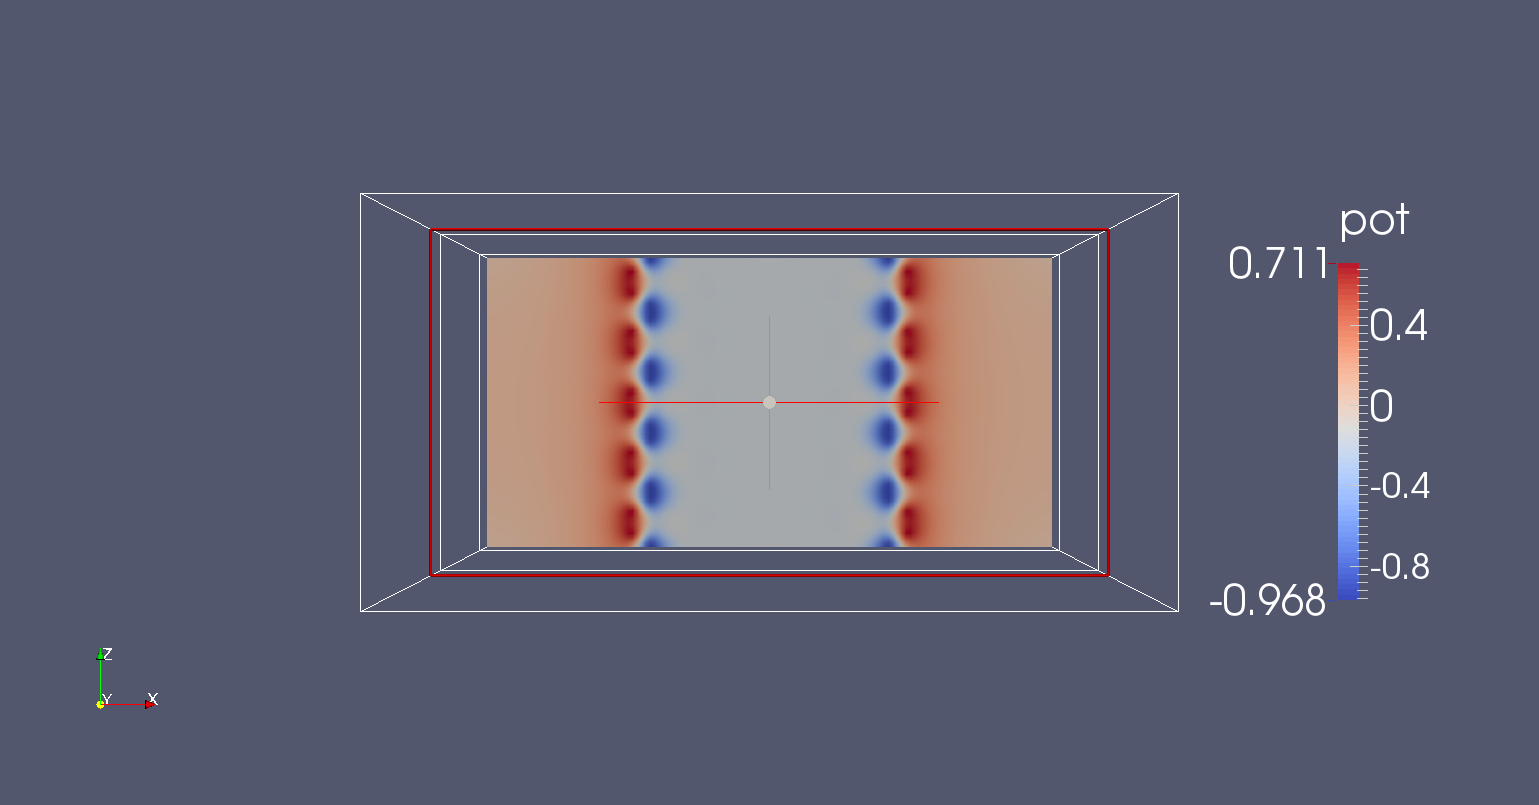
\includegraphics[width=0.800\linewidth]{clip_pot.png}
\caption{Potential profile along the nanoribbon}\label{transport:fig-clip-pot}\end{figure}

An extensive explanation of \emph{paraview} features is beyond the scope of
this tutorial. Following some easy steps, you can produce the
potential map shown in Figure {\hyperref[transport:fig-clip-pot]{\emph{\DUspan{}{Potential profile along the nanoribbon}}}} (\autopageref*{transport:fig-clip-pot}).
\begin{enumerate}
\item {} 
Open paraview and import the file \emph{pot.vtk} from File-\textgreater{}Open

\item {} 
Click on Properties -\textgreater{} Apply (Properties are usually visualised on the left side of the screen) and you should see the bounding box in the visualisation windows.

\item {} 
In the Pipeline browser select the file \emph{pot.vtk} by clicking once on it, and then select the Clip filter from Filters -\textgreater{} Alphabetical (or from the filter toolbar).

\item {} 
In Properties, click on `Y Normal' to produce a clip along the nanoribbon.

\item {} 
Click on Properties -\textgreater{} Apply.

\end{enumerate}

The plot shown in Figure {\hyperref[transport:fig-clip-pot]{\emph{\DUspan{}{Potential profile along the nanoribbon}}}} (\autopageref*{transport:fig-clip-pot}) above is the
self-consistent potential along the nanoribbon. We can see that the
charge transfer between carbon and hydrogen at the edges results in a
non-flat potential. At a first glance, the potential looks quite
homogeneous, meaning that there are no clear discontinuities at the
box boundary. This is important: being it a homogeneous ribbon, the
potential should have the same periodicity as the lattice. We can
verify this with a closer inspection by plotting a cut along a
line. We apply the following steps:
\begin{enumerate}
\item {} 
We select \emph{pot.vtk} in the Pipeline Browser and Filters-\textgreater{}Alphabetical-\textgreater{}Plot Over Line

\item {} 
From the Properties window, we select `Z Axis' and click on `Apply'

\end{enumerate}

By following this procedure we obtain Figure {\hyperref[transport:fig-plotline-pot]{\emph{\DUspan{}{Potential profile along the nanoribbon}}}} (\autopageref*{transport:fig-plotline-pot}).
\begin{figure}[htbp]
\centering
\capstart
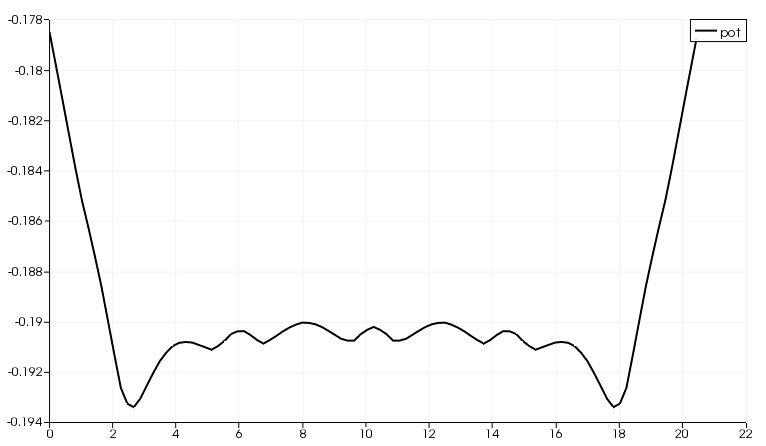
\includegraphics[width=0.700\linewidth]{plotline_pot.png}
\caption{Potential profile along the nanoribbon}\label{transport:fig-plotline-pot}\end{figure}

As you can notice, there is a discontinuity at the interface. However,
it is quite small ($\sim$ 12 meV). Defining a `perfect' interface between
the bulk semi-infinite contacts and the device region is very
difficult, especially in a semiconductor where no free charge can
contribute to screen such an interface potential. A smaller tolerance
in the self-consistent charge during the contact and the device
calculation, a finer calculation of the Fermi level (in metallic
systems) and a finer Poisson grid can decrease the discontinuity: you
should be able to reach about 1 meV, but it is difficult to go below
this value. However, as you can see in the transmission plot, as long
as the discontinuity is this small, it hardly affects the
transmission.

However, it is important for you to verify that the behaviour at the
boundaries is reasonable. Otherwise, the extended region may be too
small to allow to the relevant physical quantities (charge, potential)
to relax to bulk values. Be aware that numerical errors are
unavoidable, therefore it is important to understand their relevance
and the impact on the results. In the transmission calculation we do
not notice anything different because the energy step is close to the
mismatch at the boundaries.

After running the calculation for the pristine system, we will
introduce vacancies as we did in the non-SCC calculation. The results
should be now directly comparable to the bulk periodic SCC \emph{dftb}
calculation.


\section{SCC armchair nanoribbon with vacancy (A)}
\label{transport:scc-armchair-nanoribbon-with-vacancy-a}
{[}Working directory: \emph{transport/agr\_scc/vacancy1/}{]}

We will now calculate the SCC transmission for the nanoribbon with a
vacancy on the sublattice A, using the same input structure set up for
the non-SCC calculation. The contacts are identical to the pristine
case, therefore in the following we will only modify the extended
device calculation.


\subsection{Transmission and Density of States}
\label{transport:id4}
As previously done, the transport section must be modified in order to
account for the different number of atoms in the extended device
region:

\begin{Verbatim}[commandchars=\\\{\}]
Transport \PYGZob{}
    Device \PYGZob{}
      AtomRange = 1 135
      FirstLayerAtoms =  1 68
    \PYGZcb{}
    Contact \PYGZob{}
      Id = \PYGZdq{}source\PYGZdq{}
      AtomRange = 136 271
      FermiLevel [eV] = \PYGZhy{}4.45
      potential [eV] = 0.0
    \PYGZcb{}
    Contact \PYGZob{}
      Id = \PYGZdq{}drain\PYGZdq{}
      AtomRange = 272 407
      FermiLevel [eV] = \PYGZhy{}4.45
      potential [eV] = 0.0
    \PYGZcb{}
  Task = UploadContacts \PYGZob{}
  \PYGZcb{}
\PYGZcb{}
\end{Verbatim}

We use the same Fermi level and the files \emph{shiftcont\_source.dat} and
\emph{shiftcont\_drain.dat} as in the pristine system calculation, as the
contacts are not modified.

The \emph{Hamiltonian} block is also not modified, except for an additional
finite temperature:

\begin{Verbatim}[commandchars=\\\{\}]
Hamiltonian = DFTB \PYGZob{}
  SCC = Yes
  SCCTolerance = 1e\PYGZhy{}6
  ReadInitialCharges = No
  MaxAngularMomentum = \PYGZob{}
    C = \PYGZdq{}p\PYGZdq{}
    H = \PYGZdq{}s\PYGZdq{}
  \PYGZcb{}
  SlaterKosterFiles = Type2FileNames \PYGZob{}
  Prefix = \PYGZdq{}../../../sk/\PYGZdq{}
  Separator = \PYGZdq{}\PYGZhy{}\PYGZdq{}
  Suffix = \PYGZdq{}.skf\PYGZdq{}
  \PYGZcb{}
  Filling = Fermi \PYGZob{}
    Temperature [Kelvin] = 150.0
  \PYGZcb{}
  Electrostatics = Poisson \PYGZob{}
    Poissonbox [Angstrom] = 40.0 40.0 30.0
    MinimalGrid [Angstrom] = 0.5 0.5 0.5
    SavePotential = Yes
  \PYGZcb{}
  Eigensolver = GreensFunction \PYGZob{}
    \PYGZcb{}
\PYGZcb{}
\end{Verbatim}

A finite temperature is used to provide a finite temperature
broadening, useful if the vacancy induces partially filled gap
states. In general, temperature broadening may improve convergence and
dump oscillations in the SCC iterations.

The \emph{Analysis} block is also similar, we add the DOS calculation to
verify if we can identify a vacancy state:

\begin{Verbatim}[commandchars=\\\{\}]
Analysis = \PYGZob{}
  TunnelingAndDos \PYGZob{}
      Verbosity = 101
      EnergyRange [eV] = \PYGZhy{}6.0  \PYGZhy{}3.0
      EnergyStep [eV] = 0.025
      Region = \PYGZob{}
        Atoms = 1:135
      \PYGZcb{}
  \PYGZcb{}
\PYGZcb{}
\end{Verbatim}

As usual, you can now create the \emph{GS} and \emph{contacts} directories, copy
the \emph{shiftcont\_source.dat} and \emph{shiftcont\_drain.dat} in the current
directory and run the calculation.  The density of states and
transmission are shown in Figure {\hyperref[transport:fig-scc-vac-dos]{\emph{\DUspan{}{SCC DOS for single vacancy on sublattice A (semilog scale)}}}} (\autopageref*{transport:fig-scc-vac-dos}) and
{\hyperref[transport:fig-scc-vac-tunn]{\emph{\DUspan{}{SCC transmission in pristine (blue) and single vacancy (red) ribbons}}}} (\autopageref*{transport:fig-scc-vac-tunn}).
\begin{figure}[htbp]
\centering
\capstart
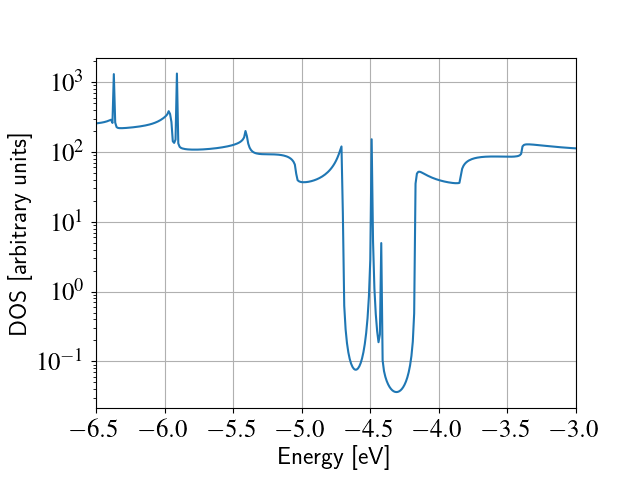
\includegraphics[width=0.700\linewidth]{scc-vac-dos.png}
\caption{SCC DOS for single vacancy on sublattice A (semilog scale)}\label{transport:fig-scc-vac-dos}\end{figure}
\begin{figure}[htbp]
\centering
\capstart
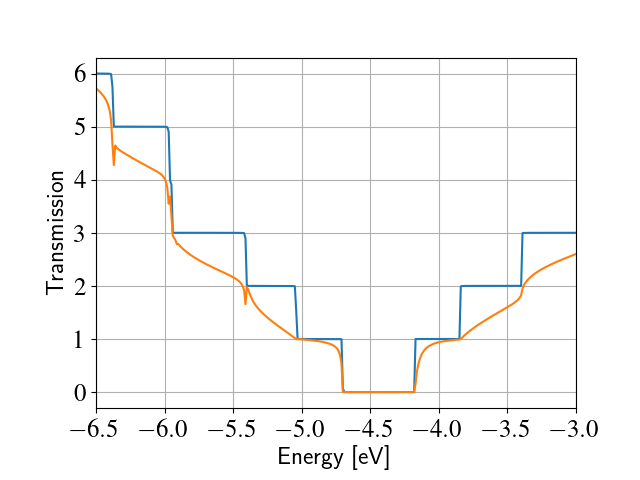
\includegraphics[width=0.700\linewidth]{scc-vac-tunn.png}
\caption{SCC transmission in pristine (blue) and single vacancy (red) ribbons}\label{transport:fig-scc-vac-tunn}\end{figure}

The vacancy states are located in the energy gap, consistently with
the periodic calculation, and that the tunneling curve is qualitative
similar to the non-scc calculation. The first conduction and valence
band are weakly affected by the vacancy which does not act as a strong
scatterer. There is no signature of resonances, as the additional
levels are located in the gap.

Note also that we previously recommended the use of large extended
regions and to verify that the potential and charge density are smooth
at interfaces. As you can see in Figure {\hyperref[transport:fig-clip-vac-pot]{\emph{\DUspan{}{Potential profile for vacancy (A)}}}} (\autopageref*{transport:fig-clip-vac-pot}), the
impurity is very close to the boundaries, resulting to a potential
profile which varies significantly close in to the boundary. It is
left to the reader to verify that the overall transmission does not
change significantly if a longer extended region is considered.
\begin{figure}[htbp]
\centering
\capstart
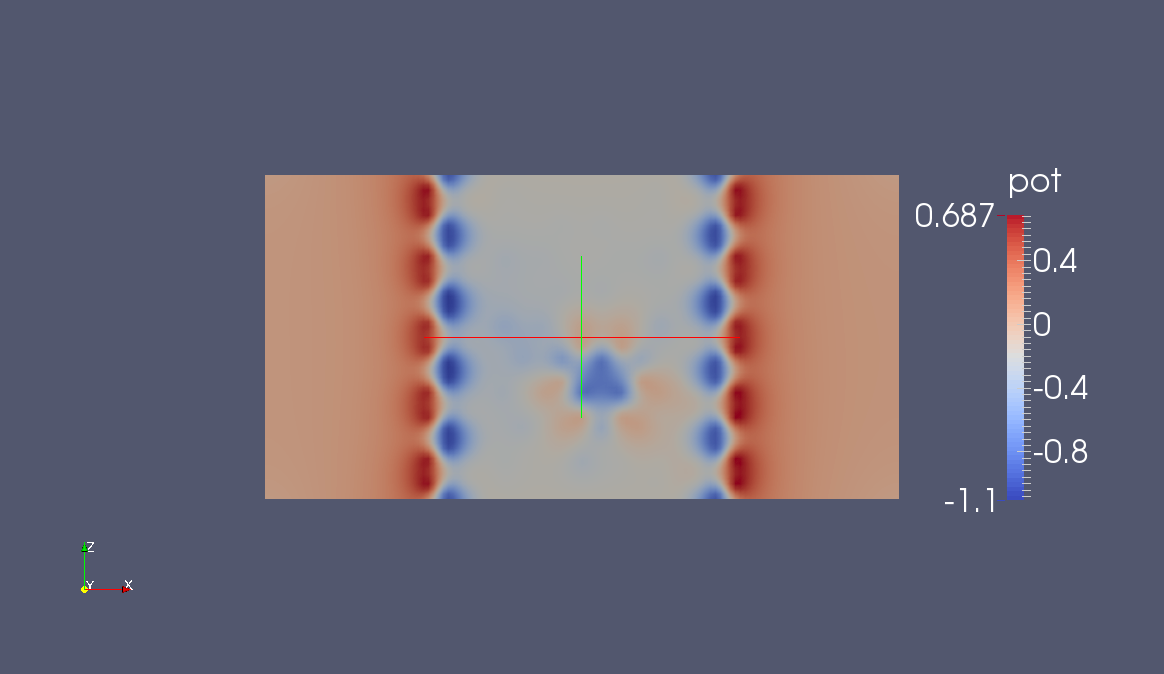
\includegraphics[width=0.700\linewidth]{clip_vac_pot.png}
\caption{Potential profile for vacancy (A)}\label{transport:fig-clip-vac-pot}\end{figure}

\newpage
\section{SCC armchair nanoribbon with vacancy (B)}
\label{transport:scc-armchair-nanoribbon-with-vacancy-b}
{[}Working directory: \emph{transport/agr\_scc/vacancy2/}{]}

We will now run the same calculation, but with the vacancy on the
sublattice B. As in the non-SCC case, the only difference with the
previous calculation is the location of the vacancy, therefore the
input file is absolutely identical. The contacts are the same,
therefore all we have to do is copy the \emph{shiftcont\_source.dat} and
\emph{shiftcont\_drain.dat} files into the current directory and run the
calculation.

The resulting transmission and density of states are shown in Figures
{\hyperref[transport:fig-scc-vac2-dos]{\emph{\DUspan{}{SCC DOS for single vacancy on sublattice B (semilog scale)}}}} (\autopageref*{transport:fig-scc-vac2-dos}) and {\hyperref[transport:fig-scc-vac2-tunn]{\emph{\DUspan{}{SCC transmission for single vacancy on sublattice B}}}} (\autopageref*{transport:fig-scc-vac2-tunn}).
\begin{figure}[htbp]
\centering
\capstart
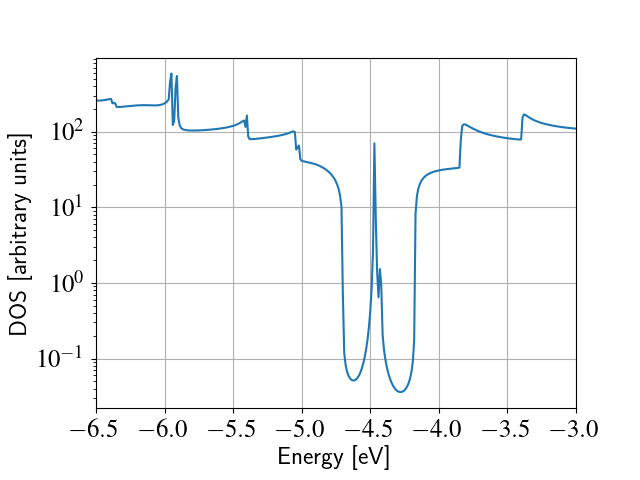
\includegraphics[width=0.700\linewidth]{scc-vac2-dos.png}
\caption{SCC DOS for single vacancy on sublattice B (semilog scale)}\label{transport:fig-scc-vac2-dos}\end{figure}
\begin{figure}[htbp]
\centering
\capstart
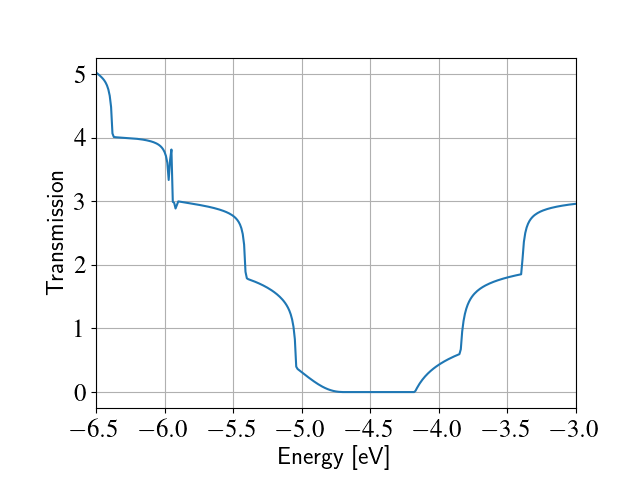
\includegraphics[width=0.700\linewidth]{scc-vac2-tunn.png}
\caption{SCC transmission for single vacancy on sublattice B}\label{transport:fig-scc-vac2-tunn}\end{figure}

We immediately notice that the Van Hove singularities are strongly
suppressed and that the valence band is almost completely
suppressed. Consistently with the picture obtained by periodic
calculation, a quasi-bounded vacancy level hybridise with the valence
band edge causing a strong back-scattering. A comparison between all
the three cases (see Figure {\hyperref[transport:fig-scc-tunn-comparison]{\emph{\DUspan{}{SCC transmission for vacancy B (green), pristine (blue) and vacancy A (red)}}}} (\autopageref*{transport:fig-scc-tunn-comparison})) shows that
the scattering probability is deeply affected by the exact position of
the vacancy. This is, in graphene nanoribbon, generally true for other
kinds of short range scattering centres such as substitutional
impurities. We can also notice that, in this particular case, the
non-scc approximation is qualitatively consistent for two reasons: the
vacancy level are not populated and the charge transfer at the edges
is not critical as the edges contribute poorly to the transmission in
an armchair ribbon.
\begin{figure}[htbp]
\centering
\capstart
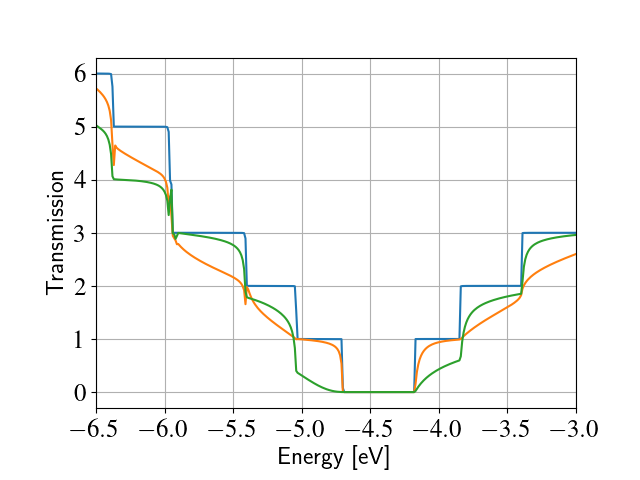
\includegraphics[width=0.700\linewidth]{scc-tunn-comparison.png}
\caption{SCC transmission for vacancy B (green), pristine (blue) and vacancy A (red)}\label{transport:fig-scc-tunn-comparison}\end{figure}

\part{Examples}

\part{Developer guide}

\chapter{{\bf\sffamily TraNaS} library}

\section{{\sffamily TTraNaS} type}

Here we describe the structure of the global container {\sffamily TTraNaS}.

\begin{itemize}

  \item {\sf Type(TTraNaSInput) :: input} -- Input container. Is not changed inside the library.
  \begin{itemize} 
    \item {\sf logical :: tPhotons = .false.}
    \item {\sf type(TPhotons) :: photons}
    \begin{itemize} 
      \item {\sf integer :: NumberModes = 0}
      \item {\sf real, dimension(:), allocatable :: Frequencies}
    \end{itemize}
  \end{itemize}
  
  \item {\sf Type(TNGF) :: ngf} -- Container for Green function methods.

  \begin{itemize} 
    \item {\sf type(TMBNGF) :: mbngf}
    \begin{itemize} 
      \item {\sf logical :: tHartreeFock = .false.}
      \item {\sf logical :: tRPA = .false.}
      \item {\sf type(TStruct\_info) :: str} -- System partitioning (as in negf{\%}str).
      \item {\sf type(z\_DNS), dimension(:,:), allocatable :: SelfEnergyR\_HF}
      \item {\sf type(z\_CSR), dimension(:), allocatable :: GreenFunctionR}
      \item {\sf type(z\_CSR), dimension(:), allocatable :: PolarizationOperatorR}
      \item {\sf real(dp) :: scc\_tol = 1.0d-7} -- SCC Tolerance.
      \item {\sf procedure :: add\_SelfEnergyR}
      \item {\sf procedure :: add\_SelfEnergyR\_HF}
      \item {\sf procedure :: get\_SelfEnergyR\_HF}
      \item {\sf procedure :: get\_SelfEnergyR\_RHF}
    \end{itemize}
    \item {\sf type(TTDNGF) :: tdngf}
  \end{itemize} 
    
  \item {\sf Type(TQME) :: qme}

  \item {\sf Type(TNEGF) :: negf} -- global container of the {\sf LibNEGF} library. 
    
\end{itemize}
}  

\part{Appendices}

\chapter*{\Large\bf\sffamily License}
\addcontentsline{toc}{chapter}{License}
\label{license:license}\label{license::doc}
This {\textsf{DFTB$^{\text{+}}$XT Guide}} is licensed under the \href{http://creativecommons.org/licenses/by/4.0/}{Creative Common Attribution 4.0
International license}.

\textbf{You are free to:}
\begin{itemize}
\item {} 
\textbf{Share} -- copy and redistribute the material in any medium or format

\item {} 
\textbf{Adapt} -- remix, transform, and build upon the material

\end{itemize}

for any purpose, even commercially.

The licensor cannot revoke these freedoms as long as you follow the license
terms.

\textbf{Under the following terms:}
\begin{description}
\item[{\textbf{Attribution}}] \leavevmode
You must give \textbf{appropriate credit}, provide a link to the license,
and \textbf{indicate if changes were made}. You may do so in any reasonable manner,
but not in any way that suggests the licensor endorses you or your use.

\end{description}

\textbf{No additional restrictions} -- You may not apply legal terms or
\textbf{technological measures}  that legally restrict others from doing anything the
license permits.

% \renewcommand{\thebibliography}{\thebibliography*}
\renewcommand{\bibname}{\Large\bf\sffamily Bibliography}

\let\oldaddcontentsline\addcontentsline% Store \addcontentsline
\renewcommand{\addcontentsline}[3]{}% Make \addcontentsline a no-op

\bibliographystyle{osa}
\bibliography{../manual/manual}

\let\addcontentsline\oldaddcontentsline% Restore \addcontentsline
\addcontentsline{toc}{chapter}{Bibliography}
\renewcommand{\indexname}{Index}
\printindex
\end{document}
